% -*- Mode:TeX -*-

%% IMPORTANT: The official thesis specifications are available at:
%%            http://libraries.mit.edu/archives/thesis-specs/
%%
%%            Please verify your thesis' formatting and copyright
%%            assignment before submission.  If you notice any
%%            discrepancies between these templates and the 
%%            MIT Libraries' specs, please let us know
%%            by e-mailing thesis@mit.edu

%% The documentclass options along with the pagestyle can be used to generate
%% a technical report, a draft copy, or a regular thesis.  You may need to
%% re-specify the pagestyle after you \include  cover.tex.  For more
%% information, see the first few lines of mitthesis.cls. 

%\documentclass[12pt,vi,twoside]{mitthesis}o
%%
%%  If you want your thesis copyright to you instead of MIT, use the
%%  ``vi'' option, as above.
%%
%\documentclass[12pt,twoside,leftblank]{mitthesis}
%%
%% If you want blank pages before new chapters to be labelled ``This
%% Page Intentionally Left Blank'', use the ``leftblank'' option, as
%% above. 

\documentclass[nobib]{tufte-book}
\usepackage{lgrind}
\usepackage{graphicx}
\usepackage{lipsum}
\usepackage{booktabs}
\usepackage{multirow}
\usepackage{moreverb}
\usepackage{alltt}
\usepackage[parfill]{parskip}
\usepackage{url}
\usepackage{array}
\usepackage{pdfpages}
\usepackage{wrapfig}
\usepackage{geometry}
\usepackage{longtable}
\usepackage{caption}
\setkeys{Gin}{width=\linewidth,totalheight=\textheight,keepaspectratio}

%% These have been added at the request of the MIT Libraries, because
%% some PDF conversions mess up the ligatures.  -LB, 1/22/2014
\usepackage{fancyvrb}

%%
% Prints argument within hanging parentheses (i.e., parentheses that take
% up no horizontal space).  Useful in tabular environments.
\newcommand{\hangp}[1]{\makebox[0pt][r]{(}#1\makebox[0pt][l]{)}}

%%
% Prints an asterisk that takes up no horizontal space.
% Useful in tabular environments.
\newcommand{\hangstar}{\makebox[0pt][l]{*}}

%%
% Prints a trailing space in a smart way.
\usepackage{xspace}


% custom page numbering
\fancypagestyle{plain}{
	\fancyhead[LE]{\thepage\quad\smallcaps}% 
	\fancyhead[RO]{\smallcaps\quad\thepage}%
}

% TODO: this was commended because we have same package above undid
% \usepackage[parfill]{parskip}

% remove paragraph indentation
\makeatletter
% Paragraph indentation and separation for normal text
\renewcommand{\@tufte@reset@par}{%
  \setlength{\RaggedRightParindent}{0.0pc}%
  \setlength{\JustifyingParindent}{0.0pc}%
  \setlength{\parindent}{0pc}%
  \setlength{\parskip}{\baselineskip}%
}
\@tufte@reset@par

% Paragraph indentation and separation for marginal text
\renewcommand{\@tufte@margin@par}{%
  \setlength{\RaggedRightParindent}{0.0pc}%
  \setlength{\JustifyingParindent}{0.0pc}%
  \setlength{\parindent}{0.0pc}%
  \setlength{\parskip}{10pt}%
}
\makeatother

%% This bit allows you to either specify onwly the files which you wish to
%% process, or `all' to process all files which you \include.
%% Krishna Sethuraman (1990).

% \setcounter{secnumdepth}{0}
% \includeonly{chap2}

\begin{document}

% % -*-latex-*-
% 
% For questions, comments, concerns or complaints:
% thesis@mit.edu
% 
%
% $Log: cover.tex,v $
% Revision 1.8  2008/05/13 15:02:15  jdreed
% Degree month is June, not May.  Added note about prevdegrees.
% Arthur Smith's title updated
%
% Revision 1.7  2001/02/08 18:53:16  boojum
% changed some \newpages to \cleardoublepages
%
% Revision 1.6  1999/10/21 14:49:31  boojum
% changed comment referring to documentstyle
%
% Revision 1.5  1999/10/21 14:39:04  boojum
% *** empty log message ***
%
% Revision 1.4  1997/04/18  17:54:10  othomas
% added page numbers on abstract and cover, and made 1 abstract
% page the default rather than 2.  (anne hunter tells me this
% is the new institute standard.)
%
% Revision 1.4  1997/04/18  17:54:10  othomas
% added page numbers on abstract and cover, and made 1 abstract
% page the default rather than 2.  (anne hunter tells me this
% is the new institute standard.)
%
% Revision 1.3  93/05/17  17:06:29  starflt
% Added acknowledgements section (suggested by tompalka)
% 
% Revision 1.2  92/04/22  13:13:13  epeisach
% Fixes for 1991 course 6 requirements
% Phrase "and to grant others the right to do so" has been added to 
% permission clause
% Second copy of abstract is not counted as separate pages so numbering works
% out
% 
% Revision 1.1  92/04/22  13:08:20  epeisach

% NOTE:
% These templates make an effort to conform to the MIT Thesis specifications,
% however the specifications can change.  We recommend that you verify the
% layout of your title page with your thesis advisor and/or the MIT 
% Libraries before printing your final copy.
\newgeometry{left=3.5cm,bottom=0.1cm}

\title{bikebump - collective urban design -}

\author{Yasushi Sakai}
% If you wish to list your previous degrees on the cover page, use the 
% previous degrees command:
% \prevdegrees{A.A., Harvard University (1985)}
% You can use the \\ command to list multiple previous degrees
\department{Media Arts and Science}

% If the thesis is for two degrees simultaneously, list them both
% separated by \and like this:
% \degree{Doctor of Philosophy \and Master of Science}
\degree{Master of Science}

% As of the 2007-08 academic year, valid degree months are September, 
% February, or June.  The default is June.
\degreemonth{September}
\degreeyear{2017}
\thesisdate{August 11, 2017}

%% By default, the thesis will be copyrighted to MIT.  If you need to copyright
%% the thesis to yourself, just specify the `vi' documentclass option.  If for
%% some reason you want to exactly specify the copyright notice text, you can
%% use the \copyrightnoticetext command.  
%\copyrightnoticetext{\copyright IBM, 1990.  Do not open till Xmas.}

% If there is more than one supervisor, use the \supervisor command
% once for each.
\supervisor{Kent Larson}{Principal Research Scientist}

% This is the department committee chairman, not the thesis committee
% chairman.  You should replace this with your Department's Committee
% Chairman.
\chairman{Pattie Maes}{Academic Head}

% Make the titlepage based on the above information.  If you need
% something special and can't use the standard form, you can specify
% the exact text of the titlepage yourself.  Put it in a titlepage
% environment and leave blank lines where you want vertical space.
% The spaces will be adjusted to fill the entire page.  The dotted
% lines for the signatures are made with the \signature command.
% TODO: snipped make title
\maketitle

% The abstractpage environment sets up everything on the page except
% the text itself.  The title and other header material are put at the
% top of the page, and the supervisors are listed at the bottom.  A
% new page is begun both before and after.  Of course, an abstract may
% be more than one page itself.  If you need more control over the
% format of the page, you can use the abstract environment, which puts
% the word "Abstract" at the beginning and single spaces its text.

%% You can either \input (*not* \include) your abstract file, or you can put
%% the text of the abstract directly between the \begin{abstractpage} and
%% \end{abstractpage} commands.

% First copy: start a new page, and save the page number.
\cleardoublepage
% Uncomment the next line if you do NOT want a page number on your
% abstract and acknowledgments pages.
\pagestyle{empty}
\setcounter{savepage}{\thepage}
% TODO: snipped abstract
% \begin{abstractpage}
% % $Log: abstract.tex,v $
% Revision 1.1  93/05/14  14:56:25  starflt
% Initial revision
% 
% Revision 1.1  90/05/04  10:41:01  lwvanels
% Initial revision
% 
%
%% The text of your abstract and nothing else (other than comments) goes here.
%% It will be single-spaced and the rest of the text that is supposed to go on
%% the abstract page will be generated by the abstractpage environment.  This
%% file should be \input (not \include 'd) from cover.tex.



Present urban planning issues require to involve the public in the urban design process, and this slow and complicated process remains the primary domain of expert planners and consultants.
Although there have been many attempts to leverage new mobile tools to engage the community.
These tools support the three stages of planning 1. data collection 2. analysis and visualization three solutions.  
Within these tools, some gather unstructured data that is hard to convert into physical interventions. Also, some applications are not designed to encourage debate and consensus building. This study will consider how a structured integrated tool will help the process of grassroots urban design.
This thesis will focus on the development of a bottom-up, crowd-sourced, urban planning tool to improve the quality and safety of urban bike lanes. A mobile application will be developed to enable non-experts to actively participate in the process of real time data collection and feedback, mapping, selection of solutions, and the establishment of priorities. The system will be evaluated using both quantitative and qualitative methods, compared to present methods on bottom up interventions.

% \end{abstractpage}

% Additional copy: start a new page, and reset the page number.  This way,
% the second copy of the abstract is not counted as separate pages.
% Uncomment the next 6 lines if you need two copies of the abstract
% page.
% \setcounter{page}{\thesavepage}
\begin{abstractpage}
% $Log: abstract.tex,v $
% Revision 1.1  93/05/14  14:56:25  starflt
% Initial revision
% 
% Revision 1.1  90/05/04  10:41:01  lwvanels
% Initial revision
% 
%
%% The text of your abstract and nothing else (other than comments) goes here.
%% It will be single-spaced and the rest of the text that is supposed to go on
%% the abstract page will be generated by the abstractpage environment.  This
%% file should be \input (not \include 'd) from cover.tex.



Present urban planning issues require to involve the public in the urban design process, and this slow and complicated process remains the primary domain of expert planners and consultants.
Although there have been many attempts to leverage new mobile tools to engage the community.
These tools support the three stages of planning 1. data collection 2. analysis and visualization three solutions.  
Within these tools, some gather unstructured data that is hard to convert into physical interventions. Also, some applications are not designed to encourage debate and consensus building. This study will consider how a structured integrated tool will help the process of grassroots urban design.
This thesis will focus on the development of a bottom-up, crowd-sourced, urban planning tool to improve the quality and safety of urban bike lanes. A mobile application will be developed to enable non-experts to actively participate in the process of real time data collection and feedback, mapping, selection of solutions, and the establishment of priorities. The system will be evaluated using both quantitative and qualitative methods, compared to present methods on bottom up interventions.

\end{abstractpage}

\cleardoublepage

% READER PAGE
\reader{Cesar A. Hidalgo}{Associate Professor of Media Arts and Sciences}{MIT Media Lab}

% TODO: snipped readerpage
\readerpage

\reader{Ethan Zuckerman}{Associate Professor of the Practice in Media Arts and Sciences}{MIT Media Lab}
\readerpage

\cleardoublepage

\section*{Acknowledgments}

This is the acknowledgements section.  You should replace this with your
own acknowledgements.

\restoregeometry

%%%%%%%%%%%%%%%%%%%%%%%%%%%%%%%%%%%%%%%%%%%%%%%%%%%%%%%%%%%%%%%%%%%%%%
% -*-latex-*-

% Some departments (e.g. 5) require an additional signature page.  See
% signature.tex for more information and uncomment the following line if
% applicable.
% % -*- Mode:TeX -*-
%
% Some departments (e.g. Chemistry) require an additional cover page
% with signatures of the thesis committee.  Please check with your
% thesis advisor or other appropriate person to determine if such a 
% page is required for your thesis.  
%
% If you choose not to use the "titlepage" environment, a \newpage
% commands, and several \vspace{\fill} commands may be necessary to
% achieve the required spacing.  The \signature command is defined in
% the "mitthesis" class
%
% The following sample appears courtesy of Ben Kaduk <kaduk@mit.edu> and
% was used in his June 2012 doctoral thesis in Chemistry. 

\begin{titlepage}
\begin{large}
This doctoral thesis has been examined by a Committee of the Department
of Chemistry as follows:

\signature{Professor Jianshu Cao}{Chairman, Thesis Committee \\
   Professor of Chemistry}

\signature{Professor Troy Van Voorhis}{Thesis Supervisor \\
   Associate Professor of Chemistry}

\signature{Professor Robert W. Field}{Member, Thesis Committee \\
   Haslam and Dewey Professor of Chemistry}
\end{large}
\end{titlepage}


\pagestyle{plain}
  % -*- Mode:TeX -*-
%% This file simply contains the commands that actually generate the table of
%% contents and lists of figures and tables.  You can omit any or all of
%% these files by simply taking out the appropriate command.  For more
%% information on these files, see appendix C.3.3 of the LaTeX manual. 
\tableofcontents
\newpage
\listoffigures
\newpage
\listoftables


% %% This is an example first chapter.  You should put chapter/appendix that you
%% write into a separate file, and add a line \include{yourfilename} to
%% main.tex, where `yourfilename.tex' is the name of the chapter/appendix file.
%% You can process specific files by typing their names in at the 
%% \files=
%% prompt when you run the file main.tex through LaTeX.
\chapter{1. Introduction}

\section{Overview}
\justify
Technology and its products influences the public norm, which then will affect the tools; both have a mutual dependence.
This thesis positions a novel tool for civic engagement within this loop of society and technology influencing each other. 

\begin{figure}[!htb]
 	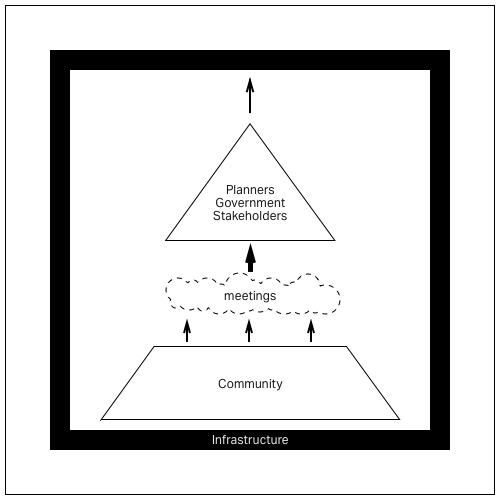
\includegraphics[width=\textwidth]{chapters/1/fig/hearings.png}               
 	 \caption[diagram: community hearings]{The pyramid divided into two parts; The top portion includes the Planners, Governors, and Stakeholders, and the \textbf{rest}. Public hearings are communication tools to let the top know the bottom. The arrow pointing to the black border indicating it changes the infrastructure, which is the boarder of the build environment and the natural environment.}
  	\label{fig:hearings}
\end{figure}

Traditionally the urban planning process accommodates public feedback through community hearings for voicing concerns from the community. The planners, government, and stakeholders will interpret the input, and plan and execute interventions that consider citizen feedback. We can think of this model as a technology to accommodate feedback once cities became too large for governance via direct democracy.

\begin{figure}[!htb]
 	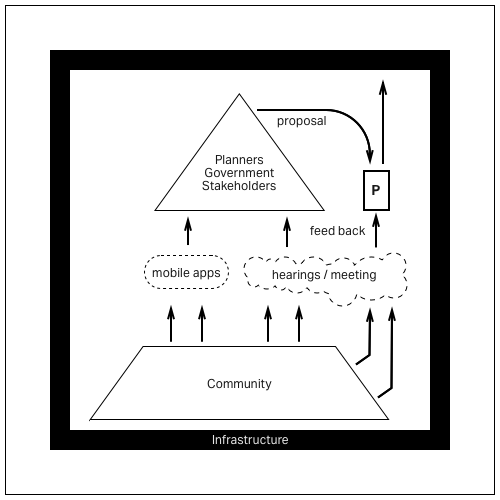
\includegraphics[width=\textwidth]{chapters/1/fig/community_engagement.png}               
 	 \caption[externalized proposal]{Demand from both the planners (wicked problem \cite{churchman1967guest}) and the community (evidence of urbanization leads to democratization \cite{woolley2010evidence} )to externalize the proposal (rectangle with P). Now citizens can provide feedback and co-design the interventions. This is the typical diagram for today's community engagement. The planners are still proposing the plans which are the primary generator of solutions.}
  	\label{fig:spin_margin}
\end{figure}

Urbanisation occurs and as cities become more dense, public demand for transparent planning increases, which results the plan to be externalized for scrutiny by the community. This increased interest in urban planning, especially transportation planning, points to the opportunity for new tools to better serve public needs.

In addition, new tools that leverage pervasive mobile communications have been developed to collect data in the form of reports and claims. These applications can be categorized as 'structured' / 'unstructured'. The majority of these applications solicit unstructured feedback, making them useful for general comments, but limiting their utility for actionable information.

These tools are mainly used for analysing the current situation, distinct from integrating (synthesis) it to one executable plan. Designers and architects have been continuously arguing that the process of analysis and synthesis should be close as possible to design properly. This mainly comes from the difference in objectives because designers and architects focuses on the integration plans rather than to provide insights. The disjoint of analysis and synthesis is one reason of failing design, since essential to the feedback process. 
Because the synthetic process in planning required domain knowledge and was hard and notably slow, the community had limited exposure to this phase of the realization of the program. Thus, community engagement processes do not have a clear distinction between the two major phases of design.

\begin{figure}[!htb]
 	\includegraphics[width=\textwidth]{chapters/1/fig/cityscope.png}               
 	 \caption[diagram: cityscope model]{The cityscope model covers the analysis through the prioritization phase. Apart from the visualization and tangible interface, it is a tool for iterating the analytical phase and synthetical phase. Note the arrow from Planners to the Plan is approval, which the plan generation is a collective collaboration from the whole community.}
  	\label{fig:diagram_cityscope}
\end{figure}

New tools have been focusing on supporting specific parts of the process, but are fragmented.
As they become mature, there is potential to have them integrated so the transition of the analytical and synthetic phase will be easier. Resulting to have more rapid iteration loops.

This thesis looks at a specific topic in urban planning: making cities more accessible to bicycles. The tool - bikebump - that allows users to passively report problems with urban infrastructure, then invites them to actively participate in planning processes to improve the urban environment. Having an integrated platform though the data collection and plan proposal is what makes this attempt novel.

\begin{figure}[!htb]
 	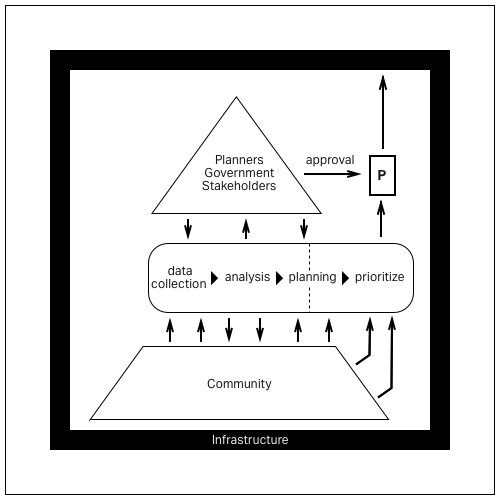
\includegraphics[width=\textwidth]{chapters/1/fig/bikebump.png}               
 	 \caption[diagram: bikebump]{The thesis investigates for a integrated tool that starts with the data collection though prioritisation.}
  	\label{fig:diagram_bikebump}
\end{figure}

The evolution of technological tools for urban planning and their relationship to public demands will be explored in the background section, before introducing the BikeBump intervention. 

\begin{figure*}[!htb]
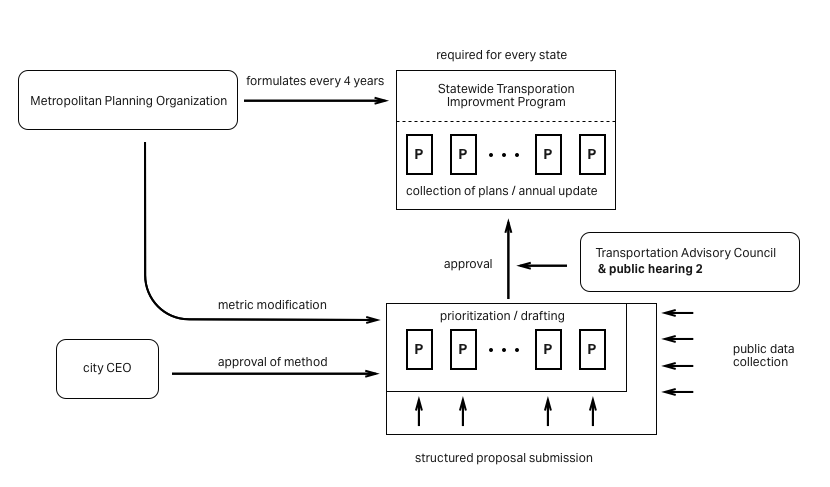
\includegraphics[width=\textwidth]{chapters/1/fig/proposed_process.png}               
 	 \caption[proposed method]{The proposed method using bikebump trying to fit the current system. The Transportation Improvement Program (TIP) is a federal requirement for each state to compile a list of executable improvements regarding transportation issues. The top of the pyramid from the previous diagrams is the Metropolitan Planning Organization and the Mayor (city CEO), given a roll of approval (which is no different from another single vote) and metric modification and engineering of plans. The improvement plans that was generated and prioritized by bikebump will undergo one last process of being approved by the Transportation Advisory Council which also tied to a public hearing.}
  	\label{fig:proposed}
\end{figure*}

Figure \ref{fig:proposed} shows a possible method form of approving bike lane improvement using this approach. There are two major differences compared to the method that is currently conducted through the United States. One, the box has inputs in two different directions from the community indicating the data collection and proposal. This is the core of this tool integrating the analytical phase and synthetic phase in one platform. Two, the planners (Metropolitan Planning Organization) and the authority (city CEO) will have a meta roll on approving and modifying the metrics to align with the long running plans. The comparison of the methodology will discussed in the Design and Implementation.
In chapter xx, I will introduce the tools and methods used for developing this web-based application, and the procedure of how it will work. The application is a web based application that runs in android devices using the standard Chrome browser.

Figure \ref{fig:how} shows the procedure of the user experience. The application has access to the phone's microphone and can detect the ring of a bicycle bell throughout the commute, saving a short sound clip of the moment before the bell ring. The sound data, the number of consecutive rings and geolocation will sent to the server for further analysis. The data will be mapped to a web browser interface that others would be able to observe. After the commute, the application will show a set binary choice questions and suggestions to ask how the situation on the street where the bell was sounded could be improved.

\begin{figure}[!htb]
 	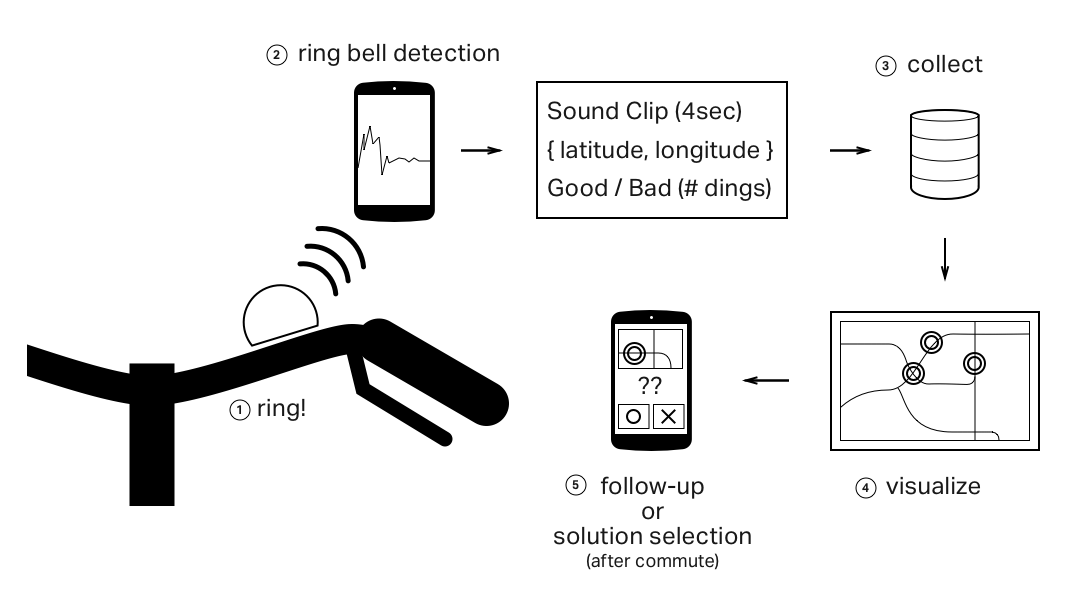
\includegraphics[width=\textwidth]{chapters/1/fig/how_it_works.png}               
 	 \caption[how bike bump works]{
 	 The flow of user interaction
 	 \begin{enumerate}
 	 \item the user rings bell if there is something worth reporting (a DING). Simple protocol of single ding indicating ``unsafe/dangerous'' and double ding indicating ``safe/pleasant''
 	 \item Smartphone detecting the frequency of the bell
 	 \item Geolocation, ``dangerous/pleasant'' value, and sound clip sent to database
 	 \item visualised to map
 	 \item user provides complementary information about the DING. Users can also propose a improvement plan by selecting a solution and the road.
 	 \end{enumerate}}
  	\label{fig:how}
\end{figure}

\section{Contribution}
The main contributions of the thesis are to connect citizens into the urban planning process through a novel technological solution. By harnessing feedback from individual bicyclists, the tool opens the urban planning process beyond mayors, professional planners and includes average citizens and collectively architect the physical environment surrounding use.
It may also help the planning side, which traditionally consist urban planners, mayors, and other stakeholders to understand the residents demand. In addition, the schema for the new urban planning support tool will externalize the process plan analysis and synthesis, which is often tacit knowledge within the planners.
The study proposes a bi-directional communication method to connect the top and bottom of the process.

% \newcommand{\repeatcaption}[2]{%
  \renewcommand{\thefigure}{\ref{#1}}%
  \caption{#2 (repeated from page \pageref{#1})}%
}


\chapter{2. Background}

This section considers the challenges of urban planning from a historical standpoint looking into the following four perspectives:
\begin{itemize}
\item Examining the physicality of democratic decision making, starting from ancient Athens to present United States town meetings.
\item Exploring the idea that urban planning connects social issues to physical sites.
\item Looking into the issues that planning experts encounter today, and examine which aspects are still critical to inherit when we have a collective tool.
\item Considering technologies that modern society can leverage and explore how it can support the complicated task of decision making.
\end{itemize}

\section{First traces of direct democracy and the scale of the city}

It is clear that modern smart phone technologies  have the potential  to support a direct democracy model in social planning. But before discussing these modern techniques, it is important to consider the underlying mechanism of how we have been planning as a crowd. Although the virtual tools have no constraints, ``scale'' is a key element in urban design. The diagram in Figure \ref{fig:diagram_primitive} is the most primitive form showing the relationship between a small community and planning, infrastructure, and buildings.
\hlcyan{A built environment is defined to be ``the human-made space in which people
live, work, and recreate on a day-to-day basis''} \cite{roof2008public}\hlcyan{, the physical layer of this human-made space is the infrastructure, which is the base of human activity.
}
Inside the built environment, we have the social environment, which is the community. The arrow from the community shows that it modifies the infrastructure.

\begin{figure}
    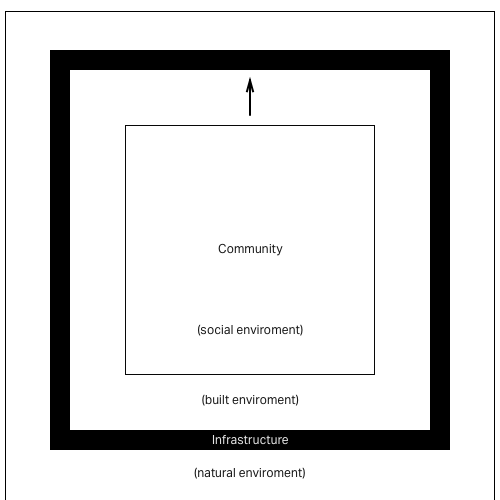
\includegraphics[width=\textwidth]{chapters/2/fig/primitive.png}               
    \caption[layers of environments]{
        The first form of a city and layers of environments. We see the community or the society in the middle,
        which is the social environment. The social environment is included in the `built environment', a physical and
        artificial region, that was first realized in Athens. The infrastructure functions as the border between this artificial
        region and the rest. The arrow indicates the community modifies the infrastructure to meet their own needs. Athens is considered
        a communal city, which the physical and artificial environment was planned first, before community was allocated.
    }
    \label{fig:diagram_primitive}
\end{figure}

This simplest form does not have any distinction within the community; it is small enough that the entire process is lead, examined, and executed from the whole.
The Athenian direct democracy is the earliest of its form of democracy that has been found documented \cite{ober2008democracy}
\footnote{It is recognized that the Athens had constantly imitate social institution from others, so it is not clear weather it is the first of its kind.}
. While we may see this as a pure form of equal political participation, it was open only to men over 18 that had military practice having the right to speak and vote during each gathering. Moreover, critics pointed out that it was biased by individual member groups which dominated the proceedings, and knowledge levels were unbalanced far from an informed decision. Despite these impurities, it is considered the very first form of direct democracy and people gathered on the hill of Pnyx as frequent as once every ten days. The hill of Pnyx had the capacity of 5000 to 13,000 people \footnote{This number of range is close to the population of the neighborhoods in Cambridge, MA \url{http://www.cambridgema.gov/~/media/Files/CDD/FactsandMaps/profiles/demo_profile_neighborhood_2016.pdf?la=en}}, and the resolved issues took immediate effect.

As it was primitive in the context of democracy, it was primitive in the sense
of urban planning as well. Before this era, cities spontaneously emerged by villages
and tribes merging and splitting organically. Athens was one of the first examples
that was artificially planned using grids,
coming from the fact it was a colony and the planner Hippodamus \footnote{often referred as the father of European urban planning.} had a task to allocate residents. Aside from the gathering and voting at the hill, there were places that men would exchange opinions and have political discussions very close to their daily lives. One such place was a room called the \textit{oikos}. This room was planned adjacent to the courtyard and was open to the public. Political theorist Hannah Arendt\cite{arendt2013human} pointed out that this early stage of the built environment and policy had an intimate relationship with each other. The wall separating the \textit{oikos} and the other rooms was called the \textit{nemein}, having a different meaning of distribution, or property, which in turn has origins to the word \textit{nomos}, which means law. Arendt emphasized that physical structures, like a wall, are political artifacts.

Lessig points out in \underline{Code: And Other Laws of Cyberspace} that there are four factors to constrain human behavior; ``code (architecture),'' ``law,'' ``market,'' and ``norm.'' \cite{lessig2009code} We see that in the age of Athens, ``code(architecture)'', and ``law'' were undifferentiated and have shared their origin.

One form of direct democracy that we can observe today is the town meetings in the northeast region of the United States. In Massachusetts, cities with a population of fewer than 6,000 are allowed to open town meetings and autonomously decide social issues. Although the types of issues are different compared to the times of ancient Greece, it is similar that the citizens pass knowledge and have interactions with one another, and collectively plan their city.


\begin{marginfigure}[{-15cm}]
  \includegraphics[width=\textwidth]{chapters/2/fig/town_meeting01.png}               
  \caption[town meetings: moderator]{a town meeting at Warren MA, 2014.11}
  \label{fig:town_meeting}
\end{marginfigure}

\begin{marginfigure}[{-5cm}]
  \includegraphics[width=\textwidth]{chapters/2/fig/town_meeting02.png}               
  \caption[town meetings: voting]{citizens show their opinion by standing up and down.}
  \label{fig:spin_margin}
\end{marginfigure}

It is said that the Roman Republic started this representative democracy, and the global majority have lived in this form of democracy since then. The world's total population has continued to rise, having both more population and density.
\hlcyan{The cost for deliberation}
\footnote{Fishkin lists the property of a deliberative discussion in five elements. \cite{fishkin2005experimenting}
\begin{itemize}
    \item Informed
    \item Balanced
    \item Conscientious
    \item Substantive
    \item Comprehensive
\end{itemize}
}
\hlcyan{increases as the number of people involved rises as well as the administrative cost for voting.}


\begin{figure}[!htb]
  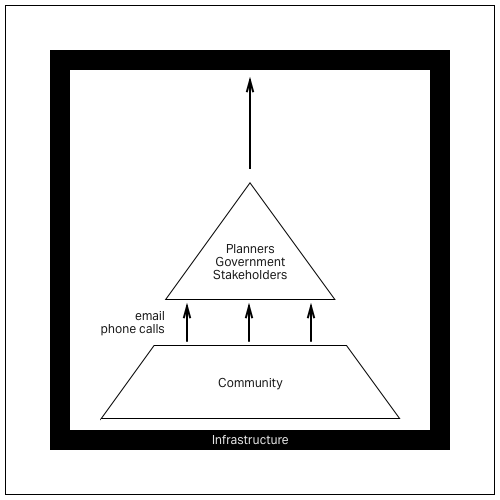
\includegraphics[width=\textwidth]{chapters/2/fig/opinion.png}               
  \caption[representative democracy]{
  As cities grew in size and density, it was no longer feasible to operate in a direct democracy model.
  The social environment changed its size into a pyramid where planners, governors, stakeholders,
  land owners plan and execute to change the city's infrastructure.
  The top part of the pyramid gathers data from the community.
  This is accomplished in various ways and media technology have been innovated to do this.
  Now the community is able to individually provide opinions to the planners.
  }
  \label{fig:diagarm_opinion}
\end{figure}

Figure \ref{fig:diagarm_opinion} shows this pyramid structure, a top down method that is elected by the broad community. Media technology, such as telephones and email, allowed the crowd to have a communication path to the top. Yet the form of communication is very different from town meetings, since these media are usually isolated, one to one methods of communications.

Methods to effectively collect opinions in a centralized way 
were invented by the planners. We can categorize these methods based on the amount of information that is exchanged (Figure \ref{fig:spectrum}). \hlcyan{The smaller the information per transaction, the easier to process, which influences the design of the tool.} For example, polls and surveys are limited in information but are easy to visualize or even directly interpret as the collective decision. The amount of data can be quantifiable by calculating the entropy\cite{shannon1998mathematical}:
\[ H = \sum_{i=1}^{n}P(x_i)log_2P(x_i) \]
\begin{figure}[!htb]
  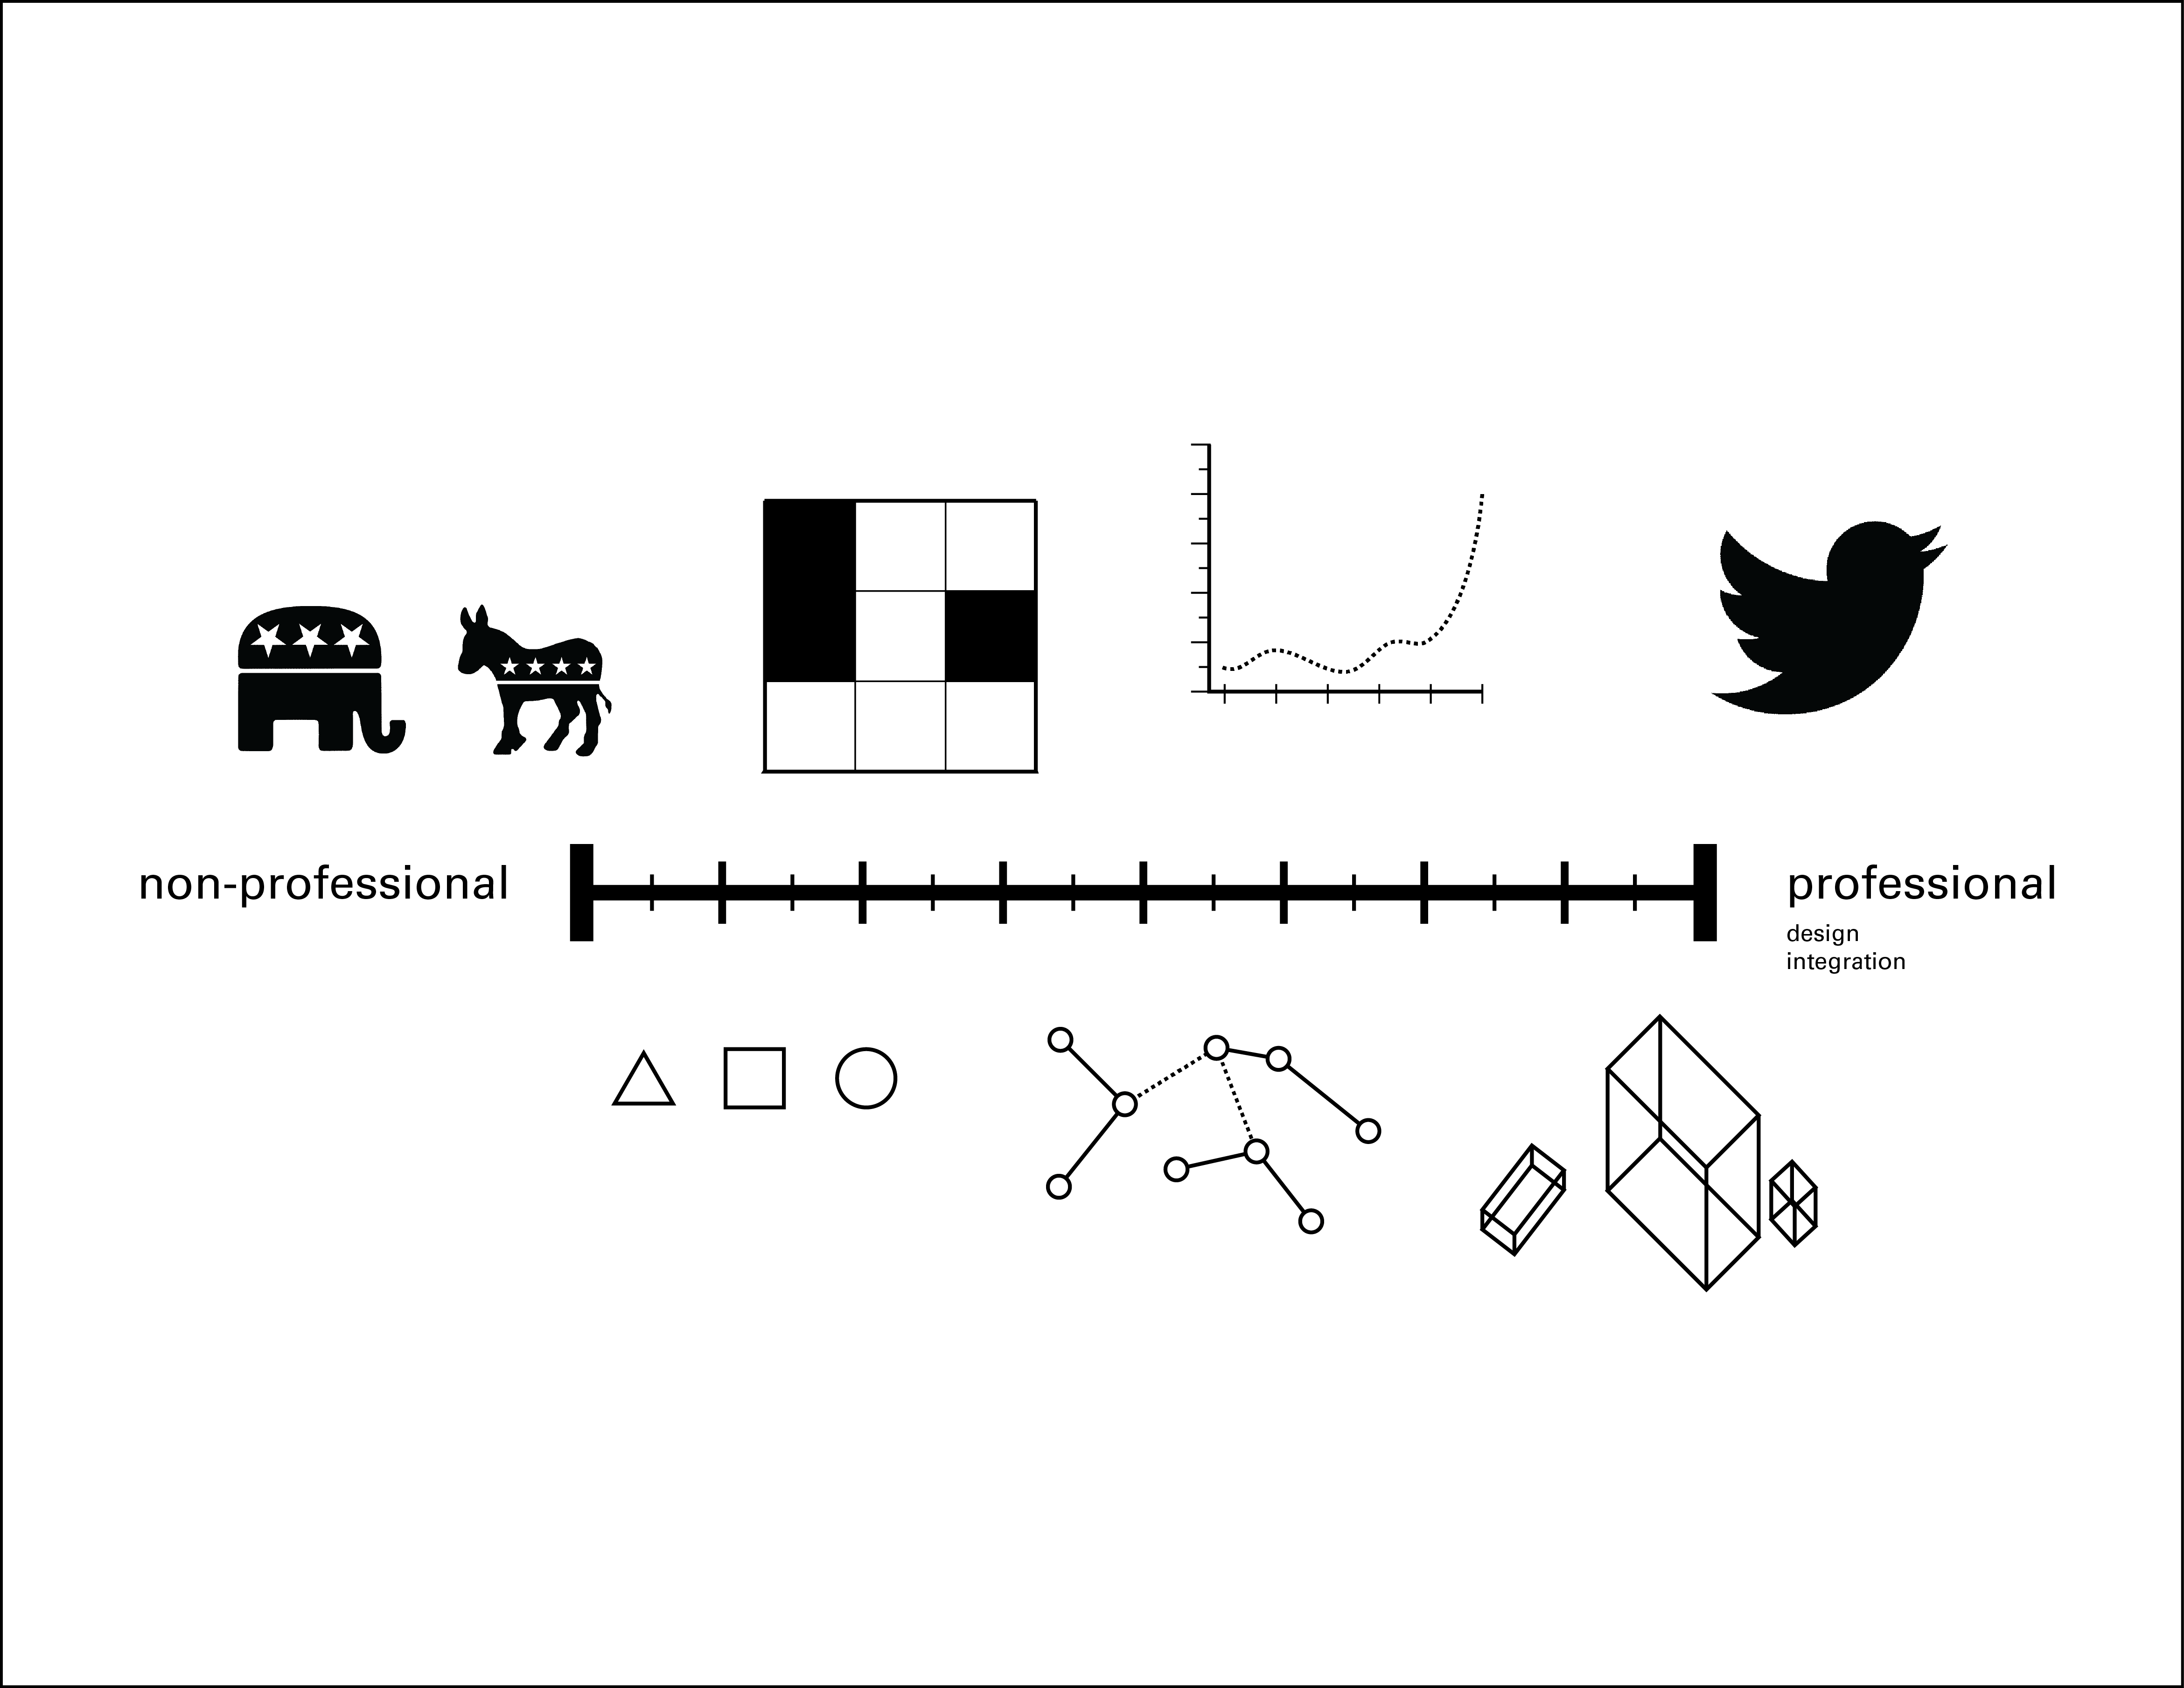
\includegraphics[width=\textwidth]{chapters/2/fig/spectrum.png}               
  \caption[number of bits per transaction]{
  The smaller the amount (bits) of information processed within one transaction,
  the easier to process. As it gets larger, it becomes unstructured data, which is hard to directly convert to a decision or
  intervention. Numbers indicate the average amount of information for each method of interaction.
  Note that that there is `unconstrained' methods, which the information is unlimited.
  }
  \label{fig:spectrum}
\end{figure}
The other side of the spectrum has the richest information and can be seen in organized events to gather people in one place which includes workshops, focus groups, \dots etc. Although these events are organized and centralized to make it effective for the head of the pyramid to listen, events are open ended, vocal, and unstructured, making it difficult to know the influence on the proposals the city made. \hlcyan{We can seek a form of interaction that is more communicative than a vote, but more structured than open discussion.} In any case, this information can be exchanged between participants, and it is influenced by what kind of media is used for this method.
\begin{figure}[!htb]
    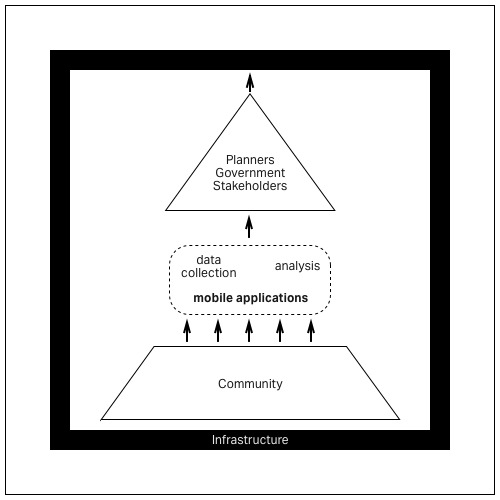
\includegraphics[width=\textwidth]{chapters/2/fig/unstructured_app.png}               
    \caption[diagram: unstructured app]{
        Modern technology enables the community to provide data in a centralized way through
        collaborative data collection and analysis.
        Compared to the methods that do not leverage the media technology,
        these are better at collecting more data at once,
        since there are no physical constraints for gathering.
        }
  \label{fig:unstructured_app}
\end{figure}


\begin{marginfigure}[{0cm}]
  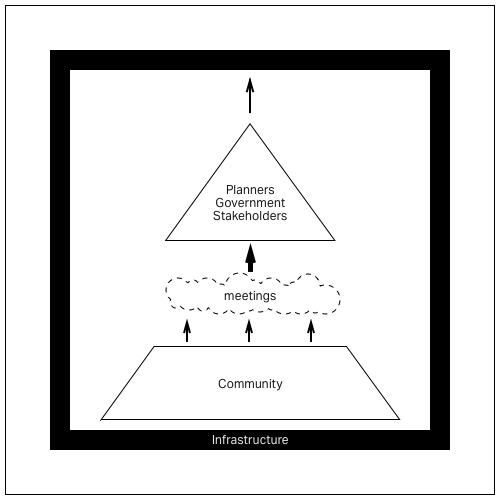
\includegraphics[width=\textwidth]{chapters/1/fig/hearings.png}               
  \repeatcaption{fig:hearings}{Urban planners started different methods of ``hearings'' to centralize input from the community. Appendix \ref{app:traditional} shows different traditional methods}
\end{marginfigure}

Different types of media technology influence these methods of hearing. Talking to each other is the least constrained, which again is unstructured, but rich.

\section{Professionals and citizens}

\begin{figure}[!htb]
  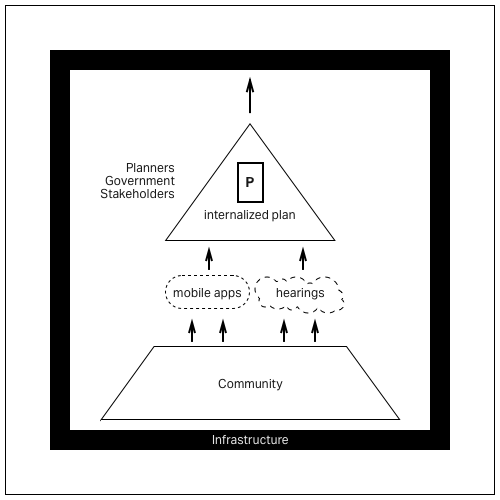
\includegraphics[width=\textwidth]{chapters/2/fig/internalized_plan.png}               
  \caption[diagram: unstructured app]{Despite the innovation in ``hearing'' methods, this state still has the plan internalized in the top section of the pyramid.}
  \label{fig:internalized_plan}
\end{figure}

Until this point, the ``plan'' or the process of planning is still internalized inside the top sector. (Figure \ref{fig:internalized_plan}) \hlcyan{Both the planner side and the community demanded to externalize this element and make it visible to everyone}.

\subsection{the planning side and the ``wicked problem''}\label{subsec:wicked}

The difficulty and complexity of social planning was addressed by Churchman which coined the term ``wicked problems'' \cite{churchman1967guest}. Churchman first points there are `tame problems', which the issues are well defined and it is clear whether the problem was solved. `Wicked problems' are the opposite, which cannot be framed in a template and are difficult to validate whether the problem was solved.  \hlcyan{We can see the frustration that planners experience in Churchman's description:}
\begin{quotation}
The lay customers are complaining because planners and other professionals have not succeeded in solving the problems they claimed they could solve.
\end{quotation}
According to Churchman, there are ten characteristics of a `wicked problem', and one of them `The social planner has no right to be wrong' challenges the position of the planner.

Similar to the contrast of `tame' and `wicked' problems, other fields of science also questioned the performance difference of professionals solving problems compared to people that are nonprofessionals. Johnson states this by the cognitive science and artificial intelligence showing results that experts perform better compared to novices while the empirical research in behavioral decision claims that \hlcyan{this is not always true}. \cite{chi2014nature} He continues that artificial intelligence focuses on structured `tame' problems like chess, where the behavioral science looks into `wicked' issues that are hard to define the aspects and detangle the influences of each of them, such as predicting the market. Hence, this has created a discrepancy of the evaluation of the performance of experts. 
\hlcyan{Johnson cites Armstrong that suggests to hire the cheapest expert, pointing their poor performance in forecasting.}\cite{armstrong1978longrange} \hlcyan{Urban planning is one of social planning, which by nature is a ``wicked problem'', which means the urban planning experts could not be guaranteed to always preform better than novices.} 

% TODO: change 'hearings' to 'community meetings'
\begin{figure}[htb]
  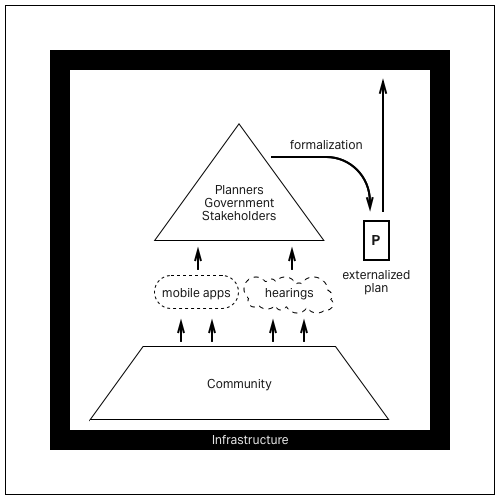
\includegraphics[width=\textwidth]{chapters/2/fig/externalized_plan.png}               
  \caption[diagram: externalized plan]{The plan has been externalized to the public. We see this by the current planning schema required to have a public meeting. (Although the strength of influence varies place to place.)}
  \label{fig:externalized_plan}
\end{figure}

\hlcyan{When planners are not able to meet public demands and are unable to predict what comes next, the gap of mistrust between public and experts increases.} \hlcyan{Especially when the value judgment is based on }Churchman's point in 1957 ``solutions to wicked problems are not true or false, but good or bad.''

One possible method to overcome "wicked problems" is to take
a collaborative approach. \cite{roberts2000wicked}
\footnote{The study examines three approaches, and concludes that the collaborative strategy is most effective.
  \begin{itemize}
\item Authoritative Strategies
\item Competitive Strategies
\item Collaborative Strategies
  \end{itemize}
}

Yet skills of collaboration are limited, especially among people who work in a traditional bureaucracy with a strong hierarchy limiting participation and team-based approaches to problem solving and decision making.

To overcome this, new tools and methods are needed to support collaboration, inform people with different perspectives, lower the administrative transaction cost, and provide a learning experience on each topic, which is exactly an effective democratic process. (Figure\ref{fig:externalized_plan})

\subsection{Democratization}

There is evidence that urbanization triggers democratic change\cite{woolley2010evidence} and as \hlcyan{urbanization is seen globally, we can assume that demands for democratization will generally increase.} Dewey advocated giving the community the power and right to collectively govern themselves, inferred that information and education are the key factors to have the community undergo decision making, and added that the `new journalist' was the one to coordinate. \cite{dewey2012public} 

He emphasizes that the `new journalist' has two central roles: verify which information is reliable; order it so the people can grasp
it efficiently.\footnote{In a modern world, a system may be able to do both using collective input.}
Shirky has pointed out that, historically, the balance between media consumption and creation from the community was dominated towards consumption, but the advent of modern communication tools and the amount of output processed from them show people also have the desire to create and share\cite{shirky2008here}. \hlcyan{We might see ``new journalism'' as a device that moderates between creation and consumption, forming a new type of system.} The challenge is to transform individual experiences, frameworks, and perspectives into a shared, understandable, and, most importantly, a transmittable area of knowledge


\begin{figure}[htb]
  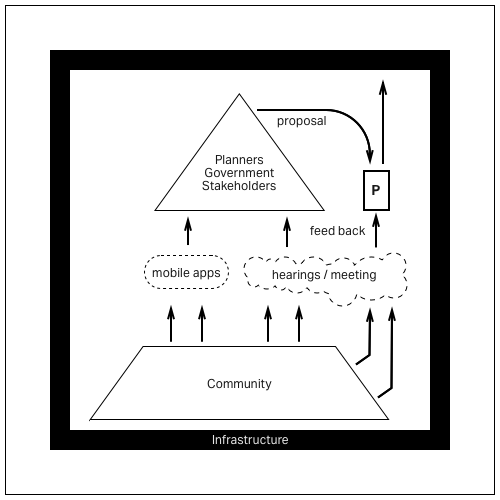
\includegraphics[width=\textwidth]{chapters/2/fig/community_engagment.png}               
  \caption[diagram: community engagement]{Community engagement that will directly influence the plan.}
  \label{fig:communityengagement}
\end{figure}

Figure \ref{fig:communityengagement} shows that people are now not only exposed the plan, but are able to provide feedback. As of 2017, it is required by Cambridge law to open a public meeting in order to obtain a permit. Again, the level of participation has been increasing and present planning procedure name this activity as the community engagement process.

\subsection{Analysis and Synthesis}
Yet the community has \hlcyan{one more step to become politically autonomous: the synthesis phase.}\hlcyan{In Athenian direct democracy, people not only voted, but proposed the topics to vote on.} In \underline{Notes on the Synthesis of Form}, Christopher Alexander clearly distinguishes that in a design procedure, there is always the analysis phase before the synthesis phase, and the two are different.


\begin{quotation}
Finding the right design program for a given problem is the first phase of the design process. It is, if we like, the analytic phase of the process. The first phase of the process must of course be followed by the synthetic phase, in which a form is derived from the program. We shall call this synthetic phase the realization of the program. \cite{alexander1964notes}
\end{quotation}

There are few attempts that distinguish these two processes. Having the premise that these two are different, there are fewer attempts to integrate them into the same platform. Figure\ref{fig:collective_design} shows one example of such a platform.
\hlcyan{The synthetic phase referred by architects was often a process done by an individual, which is a process of deciding trade offs and find the right configurations that most fits the context of a given problem. By inventing {\underline{the Pattern Language}}, Alexander created a method to synthesize an architecture plan through a deliberation process.{\cite{schulerpattern}}}

\begin{figure}[htb]
  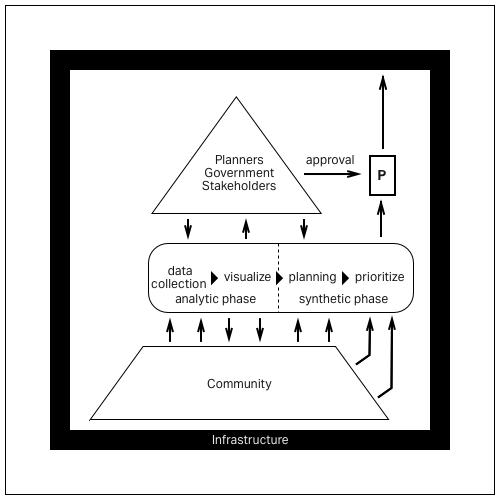
\includegraphics[width=\textwidth]{chapters/2/fig/bikebump.png}               
  \caption[diagram: integrated collective design]{Integrated design method that combines analytic and synthetic phases.}
\label{fig:collective_design}
\end{figure}


\subsection{Extending Collective Intelligence}
Artificial intelligence has been gaining attention because these technologies have advanced through the increase of available data as training sets. A substantial amount of data for training machines originates from human input, which is at the same time used for training (learn and teach) humans. Today we know this is a form of collective intelligence, which the inputs from the citizens are included in this category. Extended intelligence is a concept to acknowledge that intelligence was always a network and should incorporate both artificial intelligence and collective intelligence to utilized them mutually.\cite{pubpub:extended} Hidalgo points out that network intelligence existed from the beginning and cities are ``pockets where our species accumulates the capacity to produce information''.\cite{hidalgo2015information} He mentions that the novelty is today's technological context where computational resources have been distributed more than ever before.\cite{pubpub:whatsnew} Research says that the combination of these two types of intelligence has potential to overcome the performance\cite{baharad2011distilling} in fields that were thought to have little or no difference comparing professionals and nonprofessionals. (p\pageref{subsec:wicked}) With the collective and the artificial intelligence combined, the tool will now \hlcyan{learn} and augment the community.
% \chapter{3. Extended Examples}

\section{Traditional methods for community engagement}

\subsection{Attempts from Architects and Planners}

The objective of an Architect or a Planner is to explore many variables
until there is conversion to a single well structured solution.
aspects of a problem and consolidate into one actionable plan.
This knowledge give hints how we can integrate a participatory method
of urban design.

\textbf{Lawrence Halprin \& Charles Moore} \\
Lawrence Halprin and Charles Moore have concentrated on trying different methodologies of collaborative creative processes. For designing large scale projects, they used a large canvas to draw the plan or perspective within the community meeting, iterating through the different design possibilities. This method illustrates the designer's role of rapid prototyping.

Landscape Architect Lawrence Halprin also proposed the RVSP Cycle, a method of a collaborative creative process, which he practiced throughout his career. It is a circular diagram inspired on the compass of psyche from Jung. Table\ref{tab:rvsp} shows the elements that this diagram contains.

\begin{table}
  \centering
  \begin{tabular}{|c l | l |}
    \hline
    R & resource & data collection phase to know what is available \\ \hline
    S & score & the instruction set for the intervention \\ \hline
    V & value-action & a collective process of debating and discussion \\ \hline
    P & performance & the execution of the plan \\ \hline
  \end{tabular}
  \caption{Elements of the RSVP cycles.}
  \label{tab:rvsp}
\end{table}

The creator argues that this cycle is agnostic to where it starts or the order of execution of each element. Halprin also emphasizes that this is an endless process which changes its coordinate relative to the steps taken chronologically. (Figure \ref{fig:rvsprelative})
This relativity comes from the influence of his wife, Anna Halprin, who was a choreographer.
This behavior resembles and can be considered as a similar strategy as a search algorithm trying to look for a (sub) optimum while the fitness landscape changes at the same time.


\begin{marginfigure}
  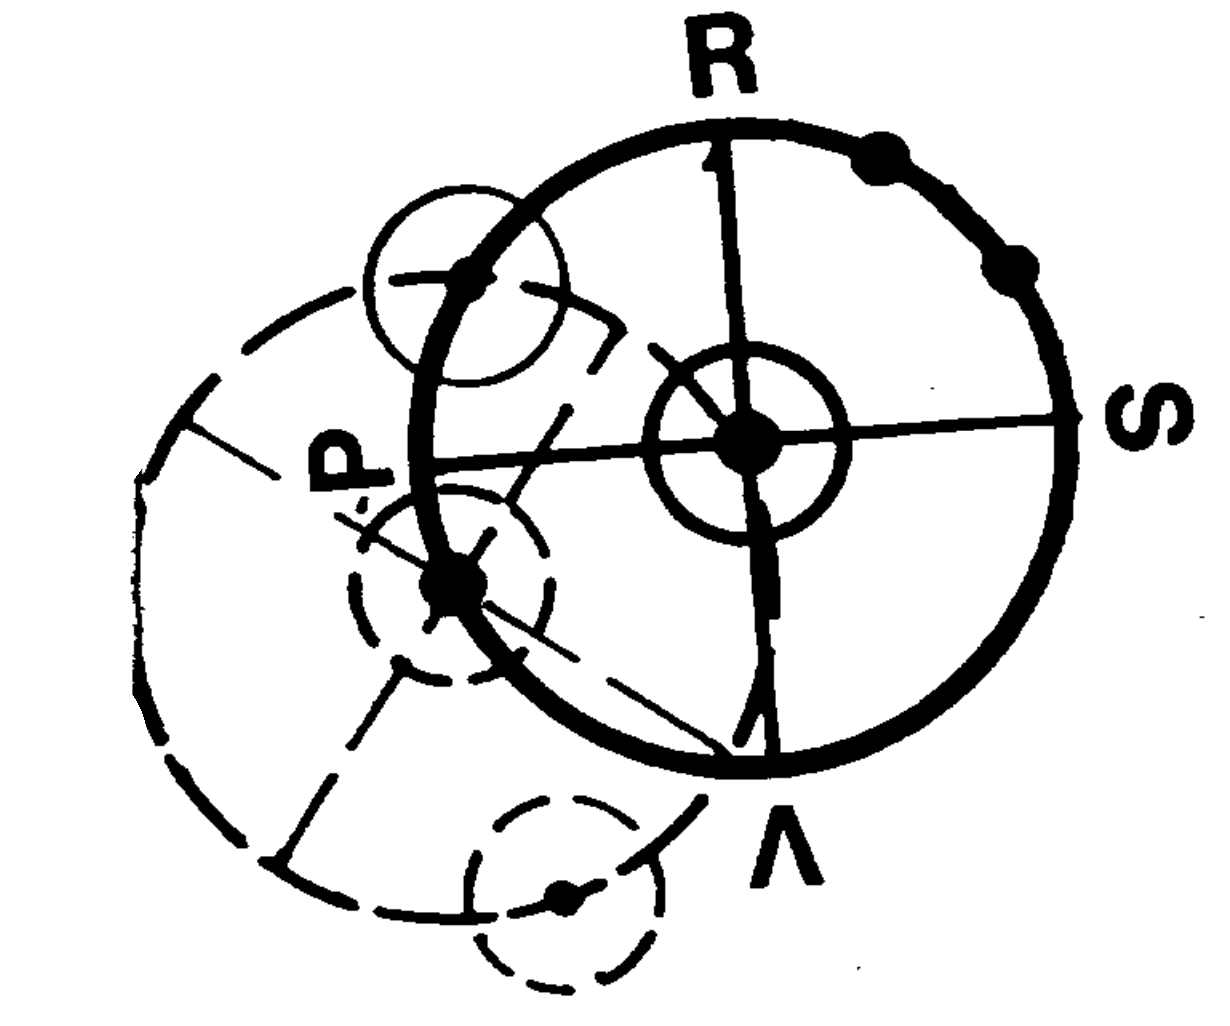
\includegraphics[width=\textwidth]{chapters/3/fig/rvsp_relative.png}               
  \caption{The RVSP cycle changes its position dynamically, relative to the previous state.\cite{halrprin1969rsvp}}
  \label{fig:rvsprelative}
\end{marginfigure}

\textbf{Arata Isozaki}\\
Architect Arata Isozaki held an exhibition in 1997 using the internet and email for planning, which is one of the earliest examples of collectively designing an urban scale project by both citizens and professional collaboration with each other. A fictitious island was the site for this design iteration with three methods for this participatory approach; each art piece named `the internet', `visitors' and `signatures.'

`The internet' was the open platform that would let opinions from the public modify the virtual plan. The total number of people connected to the web in Japan was only around 10\% of the \hlcyan{whole country's population}. The exhibition was open for gathering opinions via email and provided 3D models to modify or overwrite the existing design.
\footnote{Information Technology White Paper
\url{http://www.soumu.go.jp/johotsusintokei/whitepaper/ja/h27/html/nc372110.html}}
`Signatures' had 50 architects assigned to a site and separately planned one of their previous architectural pieces without the considerations that are usually sorted out, such as orientation and size. The initial layout plan triggered problems that would need negotiation between adjacent architects to `fit' their design properly. 
`Visitors' focused on the chronological aspect of collaborative design. It had a chief architect that supervised one district for a total of two weeks, passing it to the next architect after their turn. This work flow has similarities in today's software development, where people collaboratively develop software by forking code made by peers. The architects were encouraged to collect data from the internet. This exhibition was not only novel because of using the internet and email, but was an experiment on how we collaborate and interact using these new techniques.

\hlcyan{Each dealing with mass communication(=`the internet'), negotiation with peer neighbors(=`signatures'), and chronological collaboration(=`visitors'), we see that this exhibition takes collaboration as the central factor, experimenting what will happen when modern technology has been introduced to it.}


\subsection{Browser based applications}

\hlcyan{Browsers are a type of software that arguably have had the most money and effort involved in their development.} Yet `browsers' are particular in ways that are cross platform, including different devices from smart phones to desktop work stations. The following are the web applications I have developed for participatory design.

\textbf{Nigechizu -Shortcut Evacuation Planning \hlcyan{for Tsunamis}-}

\begin{figure}[htb]
  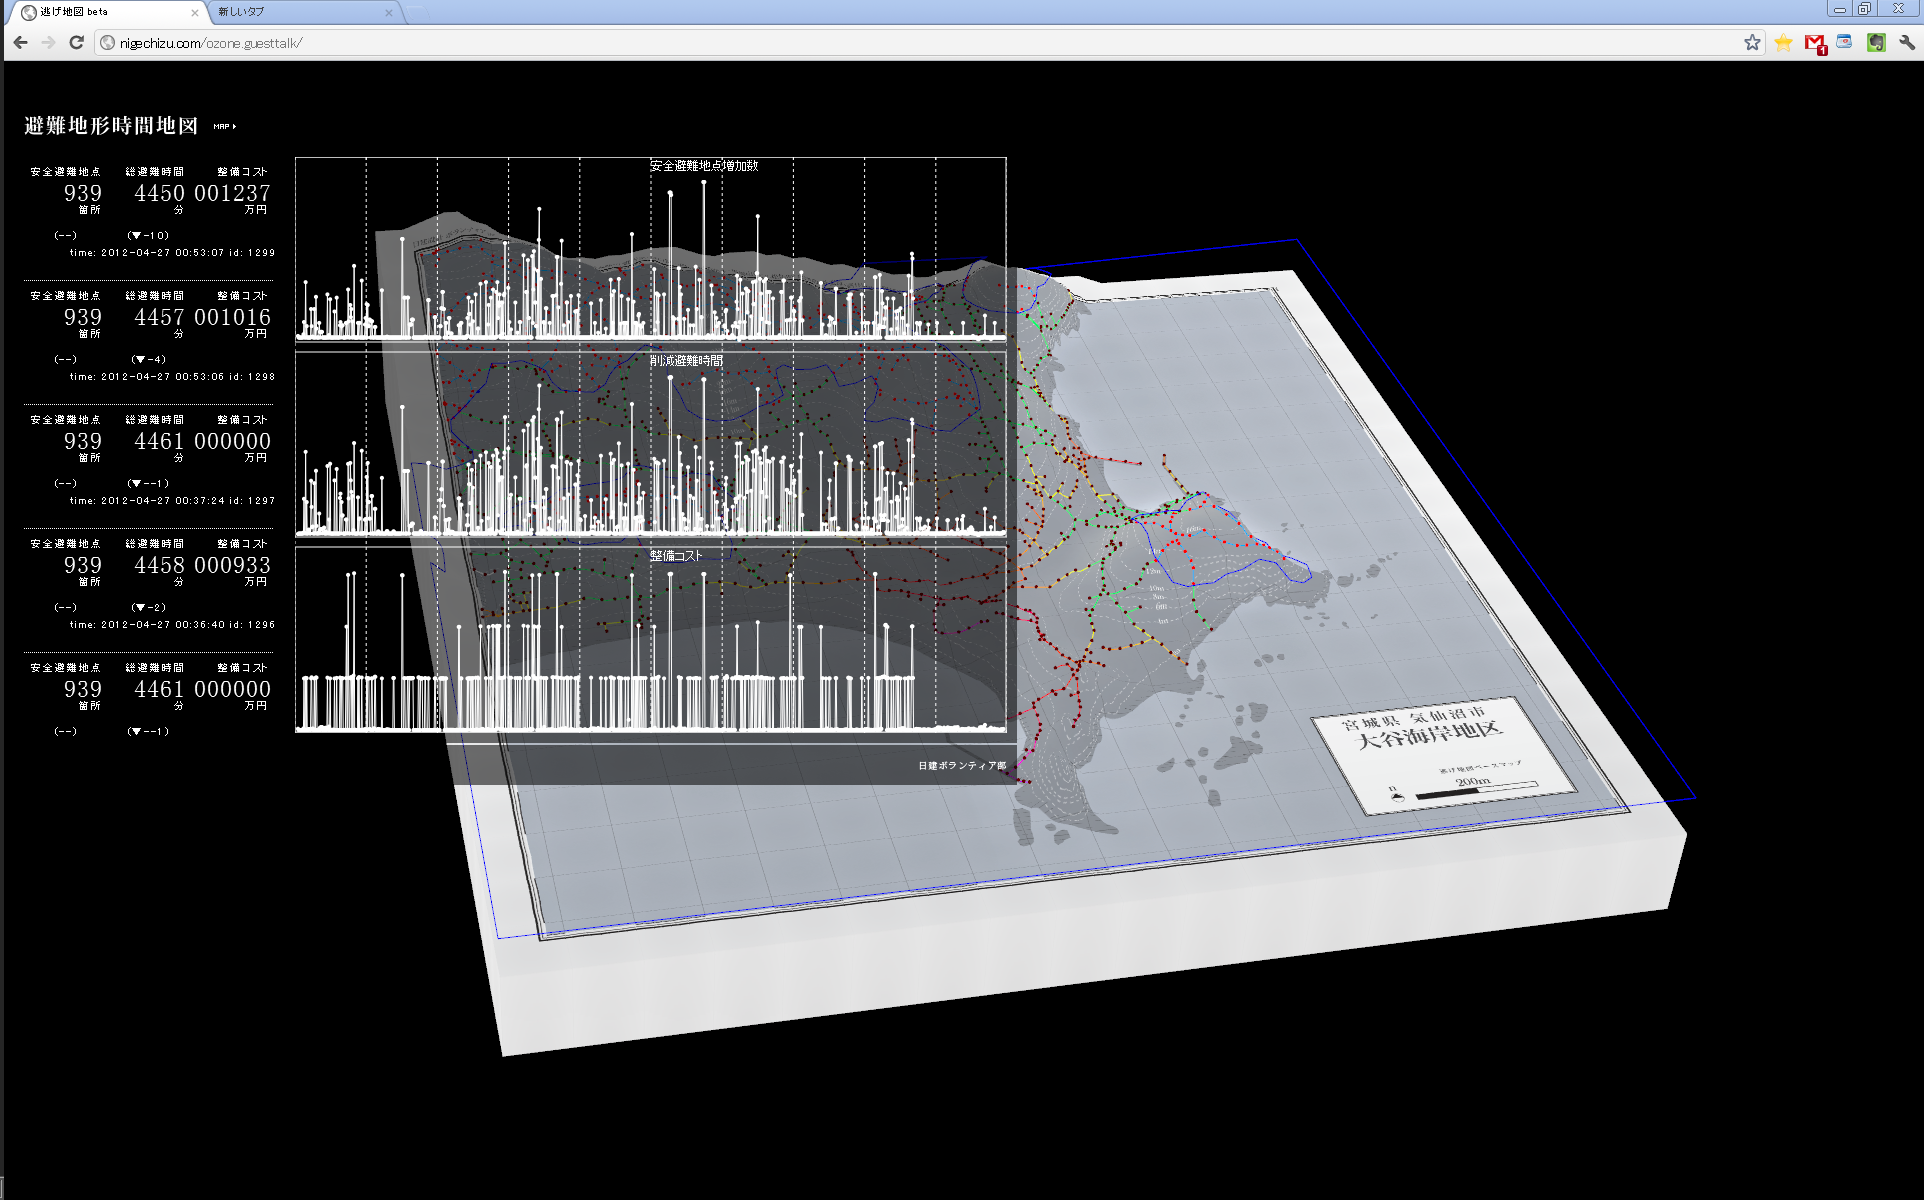
\includegraphics[width=\textwidth]{chapters/3/fig/nigechizu002.png}               
  \caption[nigechizu]{Web based short cut planning tool: Created for workshops to learn the risks of tsunamis and how to evacuate.}
  \label{fig:nigechizu}
\end{figure}

As a reaction of the tsunami damage from the 2011 Tohoku earthquake and tsunami, I have created this tool to engage citizens affected by this disaster.

This web browser based tool starts by visualizing the risk of a tsunami coloring the paths depending on the duration for evacuation.
\footnote{This was calculated by a normal walking speed of an elderly citizen, taking the shortest path to the closest high enough altitude.}
After the first strike of the tsunami, people constantly wanted to know which direction to escape because it was sometimes not obvious given the \hlcyan{complex} terrain of the Tohoku region. The second feature was to let the community choose how to create shortcuts. Since shortcut paths reduce the time for evacuation, selecting two points and connecting them increases the area's safety level as a whole. The significance of this app is enabling people to choose two points to connect, unlike voting for a particular configuration. The trials were recorded in the server to be superimposed to get the most popular positions that needed to be connected.

\begin{marginfigure}[{0cm}]
  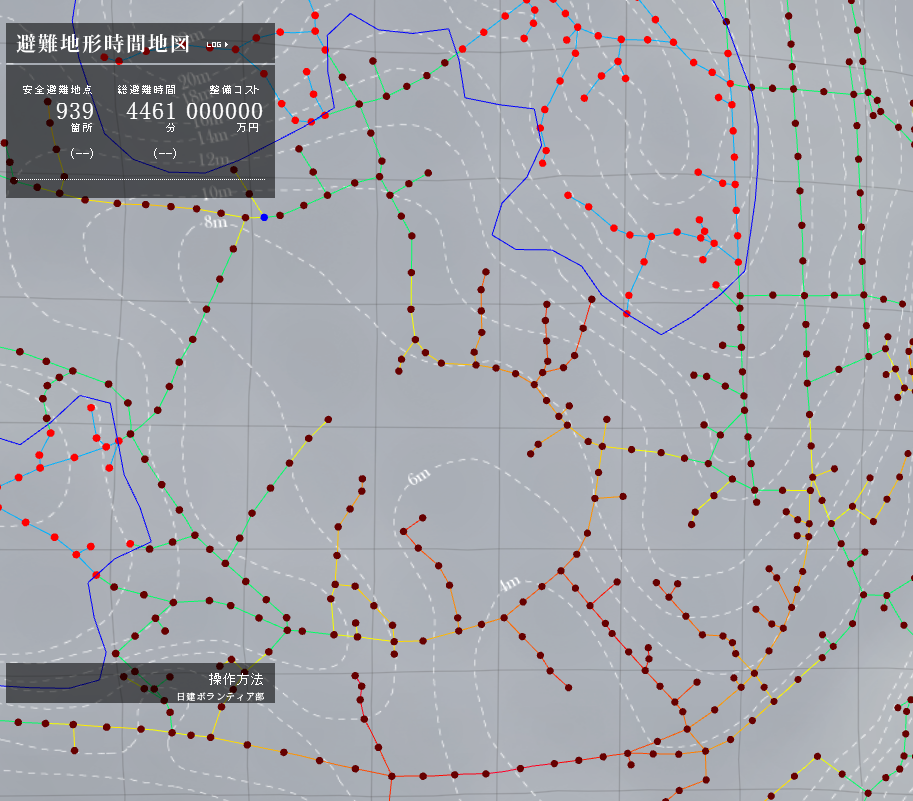
\includegraphics[width=\textwidth]{chapters/3/fig/nigechizu001.png}               
  \caption[zoom in nigechizu interface]{Users will connect two points to create a shortcut to decrease the overall evacuation time.}
  \label{fig:nigechizu}
\end{marginfigure}

\begin{marginfigure}[{0cm}]
  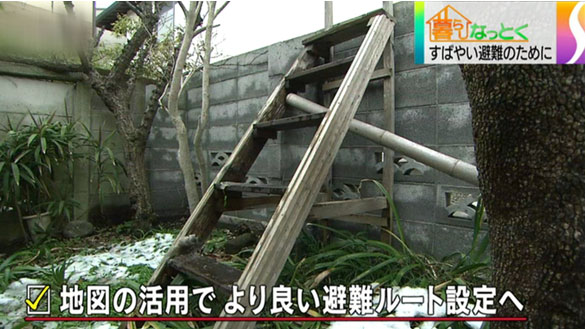
\includegraphics[width=\textwidth]{chapters/3/fig/nhk_kamakura.jpg}               
  \caption[collective collaboration]{After one of the workshops neighbors
  negotiated with each other and installed a wooden staircase to be used as
a general asset for emergency evacuation. \url{https://www3.nhk.or.jp}}
  \label{fig:nigechizu}
\end{marginfigure}


\textbf{LMN Architects -distributed version controlling in 3d
models-}

This example is also a 3d modeling application in a web browser, and every model is connected forming a network. The connection of two models is the inheritance, where the participants choose a preexisting model as a reference and start modeling on top.  The user submits a 3d model, which is a large amount of data compared to voting or connecting dots, and often thought of as unstructured data. The application saves the 3d model into a data structure that could apply a diff algorithm to make the 3d model comparable and calculate the similarities between two models visualizing the strength of the connection.

\begin{figure}[htb]
  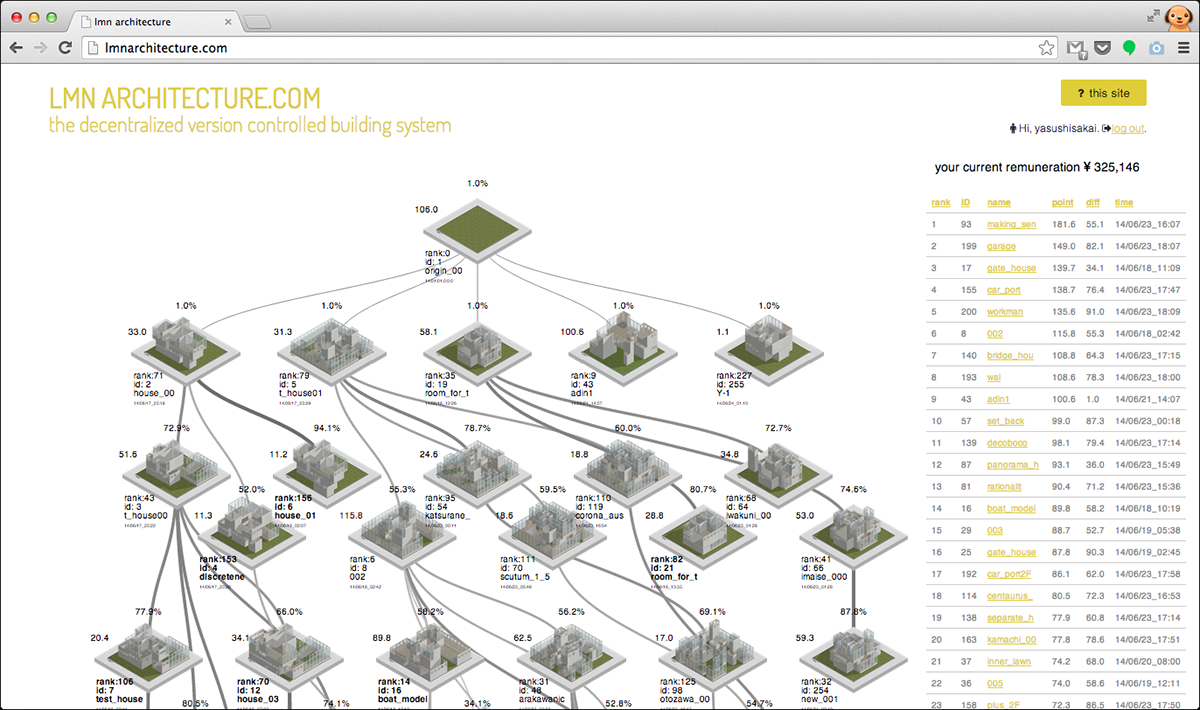
\includegraphics[width=\textwidth]{chapters/3/fig/lmn_004.png}               
  \caption[LMN:web based distributed modelling]{Web based distributed modeling.}
  \label{fig:lnm}
\end{figure}

\begin{marginfigure}[{0cm}]
  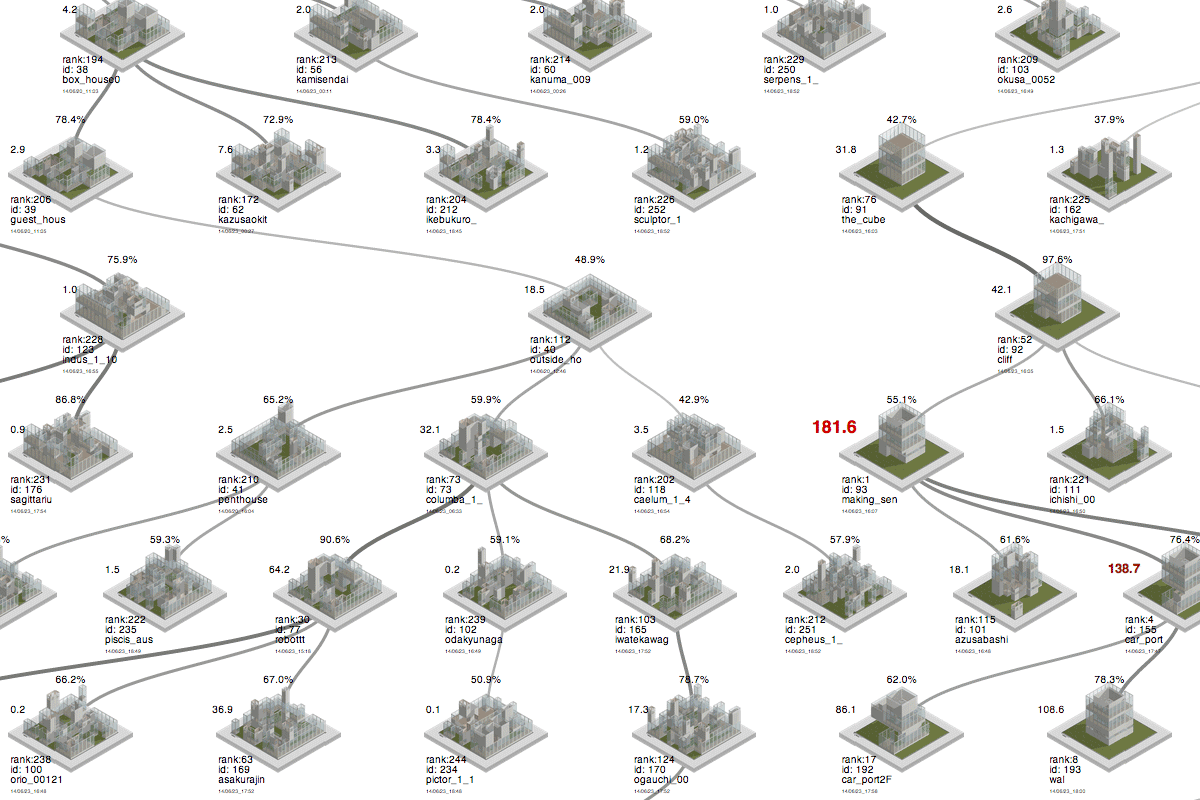
\includegraphics[width=\textwidth]{chapters/3/fig/lmn_000.png}               
  \caption[LMN:net work of models]{Each model starts with a preexisting model and revises it.
Thus, every model is connected, having the similarities calculated by the diff algorithm.}
  \label{fig:lnm_zoom}
\end{marginfigure}

\begin{marginfigure}[{0cm}]
  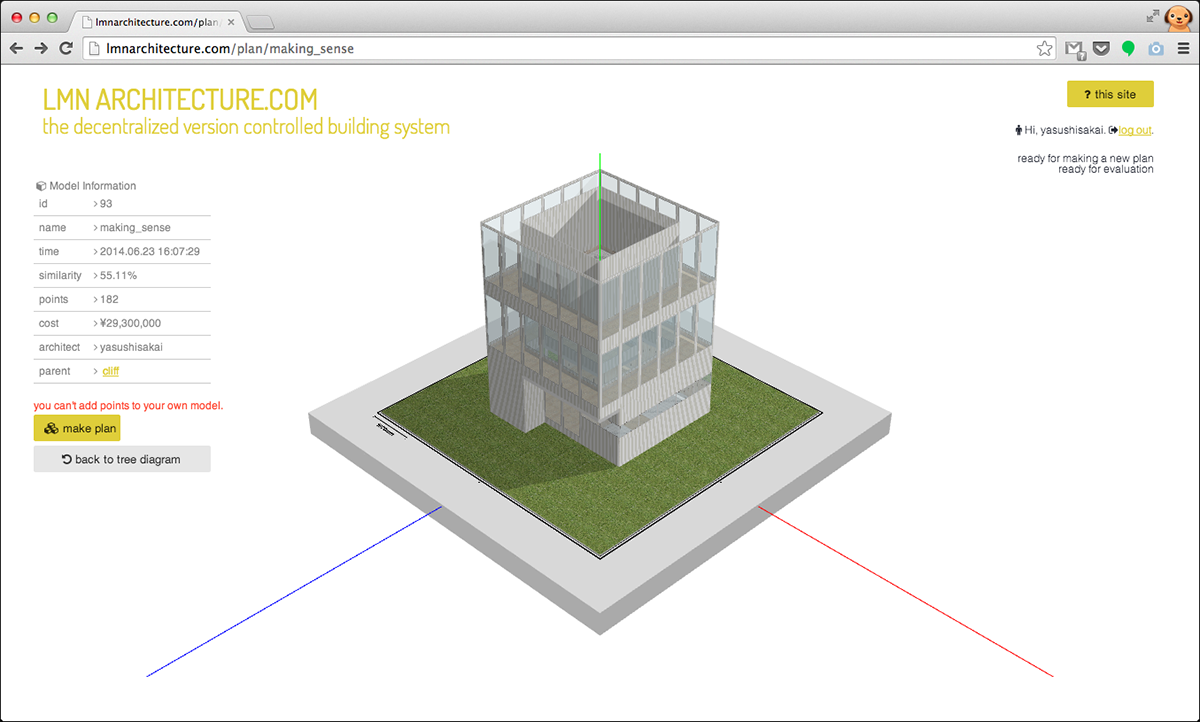
\includegraphics[width=\textwidth]{chapters/3/fig/lmn_006.png}               
  \caption[LMN: modeling inside the browser]{Every model is created using the web browser.}
  \label{fig:lnm_create}
\end{marginfigure}

\textbf{PlacePulse}\\
Place Pulse\footnote{\url{http://pulse.media.mit.edu/}}\cite{salesses2013collaborative} developed by the Collective Learning Group in MIT Media Lab, is a collective effort to map our perception about the city by selecting one image out of two. 10 The amount of information sent per interaction is the smallest in this section, yet has collected more than 1.4 million clicks\footnote{as of August 2017}.

\subsection{Mobile Applications}

\textbf{SeeClickFix}\footnote{\url{https://en.seeclickfix.com/}}\\
\hlcyan{SeeClickFix is a mobile application that is similar to calling the number `311' when citizens demands to report non-emergency maintenance issues. Originally developed for the city of New Haven and has now expanded for more than 300 cities Reporters can submit text and pictures, which is unconstrained. Although not clearly specified, the reports focus on maintenance issues, and less about the planning and changing the city.}

\textbf{Waze}\\
Waze is a driving navigation application, which uses the status of other drivers using the same application. Each driver can passively send the location and speed of the car, or actively contribute to marking the road if there is something worth noting to other drives. Each data is structured. This distributed traffic monitoring is an example of collective analysis, creating mutual benefit and a sense of inclusion between complete strangers who do not share any identity except being drivers. The objective of this application is to form this collective intelligence; there is no connection to any planning procedure.

\textbf{Street Bump} \\
Street Bump developed by the new urban mechanics, is a mobile application that gathers accelerometer data while driving. It is a passive data collection method\footnote{where people do not proactively interact with the data} which is similar to waze, but focused on detecting potholes. The application introduces one question of whether or not we should have the human's fuzziness in the data. In one way, the accuracy of detecting a pothole is a matter of engineering, thus a `tame' problem. Yet we do not know if the human subjects actually cares or feels the pothole is important. In severe cases, people may avoid to step on a pothole, which observation of human behavior is crucial for sensor oriented projects. 
\cite{o2013exploiting}

\textbf{Action Path}\\
Action Path,\footnote{\url{http://actionpath.org/}} \cite{graeff2014crowdsourcing} developed at MIT Center for Civic Media, is a mobile application that shows notifications when a user enters a predefined geolocation and asks questions on urban issues tied to that geolocation. The application provides agency to the citizens and creates data to represent the collective opinion. The interaction with the user produces one of the smallest amounts within this section.

\subsection{Augmentation of Offline community engagement by online tools}

\textbf{Tangible Interfaces: CityScope, Finding Places}\\
City Scope is a platform for people to gather and \hlcyan{build consensus using a device that incorporates data projections}, a tangible interface, and real-time simulation. Multiple projects have advanced using this platform collaboration with different cities and universities. Each project has a different focus, hence the content\footnote{What to visualize/project, type of simulation, who to engage, objective.} has varied.

Finding Places uses City Scope to prove a space for discussing the issue of placing immigrants who’ve come to Hamburg, Germany\footnote{Germany received more than 1.2 million refugees in 2015.}. Using a City Scope table, a total of 34 workshops were conducted to discuss the best place to open room for those seeking asylum. Each session took 2 hours with on average 11 people participating.

This tool covers the analytic phase and synthetic phase and enables people to have real-time feedback running simulations showing potential implications of the population increase. It is a structured tool since users manipulate color coded Lego bricks to run each simulation. On the other hand, the discussion held over the table is rich and vocal.

\begin{figure}[htb]
  \includegraphics[width=\textwidth]{chapters/3/fig/cityscope.png}               
  \caption[diagram: cityscope]{Changing Places City Scope Platform.}
  \label{fig:diagram_cityscope}
\end{figure}

\textbf{Community PlanIt} \\
\hlcyan{Community PlanIt\footnote{\url{https://elab.emerson.edu/projects/civic-media/community-planit}} developed by the Engagement Lab is gaming platform to support civic participation in planning projects.
The platform asks questions or missions to the participant inducing conversation with each other or manifest each others vision for the city. The platform can be used parallel with public meetings that will foster the deliberation process of the event.
}


\textbf{Cambridge participatory budgeting} \\
\hlcyan{Participatory budgeting originated in 1989 Brazil, is a bottom up method that people propose and decide how to spend a portion of public tax revenue. Cambridge has been conducting this project, with browser apps augmenting the process. The application has two views: the map and the list. Them map is plot of different proposals that was submitted by other citizens. Users can explore different proposals within their neighborhood. The list has the same information but is sorted by the attention the project has collected.
}

\textbf{coUrbanize}\footnote{\url{https://courbanize.com/}} \\
/hlcyan{This is online platform for urban planners and real estate developers to post their projects and host discussions to gain feedback. The tool is more a platform to list different development projects.}

\textbf{tools from delib} \\
\hlcyan{Delib \footnote{\url{http://www.delib.net/}} developed a series of online platforms for different occasions necessary for planning and community engagement: `Dialogue' is for project manifestation for gaining feed back of plan proposals, `Citizens Place' is for consolidating questionnaires and online consultations, and `Budget Simulator' is for engaging citizens to gain insights on projects with budgets taken into consideration.}


% %% This is an example first chapter.  You should put chapter/appendix that you
%% write into a separate file, and add a line \include{yourfilename} to
%% main.tex, where `yourfilename.tex' is the name of the chapter/appendix file.
%% You can process specific files by typing their names in at the 
%% \files=
%% prompt when you run the file main.tex through LaTeX.
\newcommand{\repeatcaption}[2]{%
  \renewcommand{\thefigure}{\ref{#1}}%
  \captionsetup{list=no}%
  \caption{#2 (repeated from page \pageref{#1})}%
}

\chapter{4. Design and Implementation}

\section{Case Study: bikebump}
To test a system of that handles data collection through plan
prioritization, an application for improving bike lanes was selected for a
case study. Using bikes for commute has been a trend through recent years
though the U.S., one consensus shows that there was a 3\% increase of
people choosing bikes for everyday transportation from 2010 to 2013 and is
close to double compared to the year 2000.\cite{debra2016onemillion} We can see the trend of cities investing on improving bike lanes are in sync especially in dense city areas. New York city has had 400 miles of cycle path renewals starting from the 2000s. The field of public health public health supports this by research by showing investment on bike lanes are efficient compared to other public health interventions.

\subsection{Urban Planning}
Urban planning interventions tend to have exceptional cost impact, yet the process for deciding which to execute is also long and tedious. Because of this slow process and cost impact, it is difficult to make the proposal creation as a learning process. 
In the united states, the construction cost for a highway is 8million to 10 million USD per mile, where one of the most expensive bike lanes will cost 445,000 USD per mile. Bike lanes relatively inexpensive, starting with simply paint. Moreover these interventions are reversible, which enables to iterate for try and error.

It is certain that like painting bike lanes are cheap reversible thus may be able to make the process fast, but some interventions are expensive and requires lots of domain knowledge and engineering which inevitably will be a slow process. It is difficult to design or even reach a consensus within the community, because of the duration, a tentative pole may not directly reflect the demand of citizen when the construction is actually completed, especially where people tends to move frequently. Yet there are examples that the demand of such long and costly infrastructure is decreasing, since this relates to different types of transportation people uses. If the trend of the number of cars decrease continues and multi modal transportation is accepted, light interventions such as bike lane improvements will raise the share, supported by the trend of the increase of population density, the cost impact per population will be decrease.

\section{Current Method for Changing bike related infrastructure}

The Transportation Improvement Program is a federal requirement for each state listing improvements for transportation all needs. This is the standard way though U.S. and bikeway improvements are included.

\begin{figure*}[!htb]
  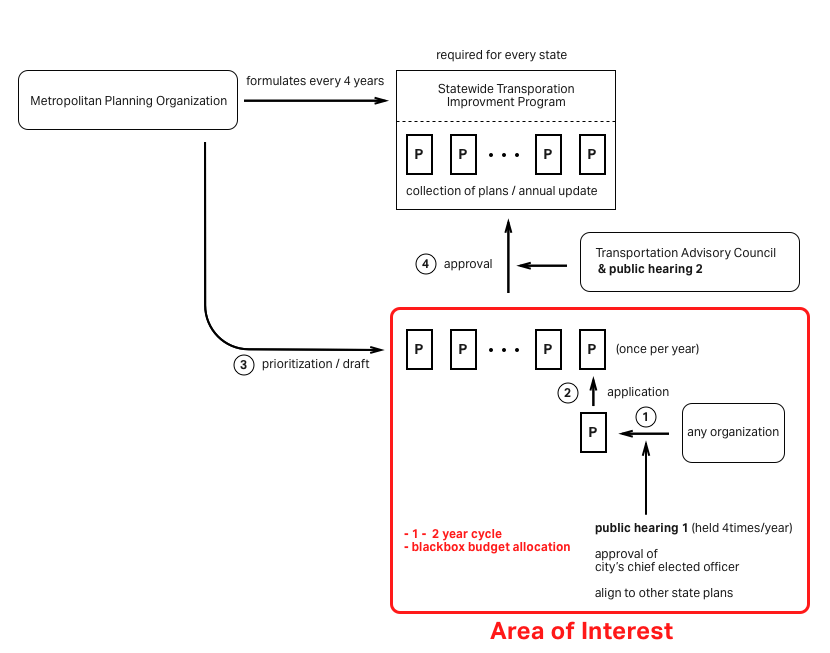
\includegraphics{chapters/4/fig/tip_process.png}               
  \caption{TIP(Transportation Improvement Program) required by each state. \url{https://www.gpo.gov/fdsys/pkg/USCODE-2011-title23/html/USCODE-2011-title23-chap1-sec135.htm} 
  }
  \label{fig:tip_process}
\end{figure*}

\begin{enumerate}
\item The process starts with a the city level required to have least one public hearing, and approval of the city's mayor. This needs to be aligned to be aligned with the state level manifesto.
\item After meeting the city level criteria, it is scrutinized by the local office of Metropolitan Planning Organization. The MPO evaluates and engineers the proposal to a executable plan. The MPO also prioritises the plans.
\item The list of plans will be undergoing a second public hearing and discussed with the Transportation Advisory Council.
\item Once approved the proposal will be listed into one plan inside the Statewide Transportation Improvement Plan.
\end{enumerate}

\begin{figure*}[!htb]
  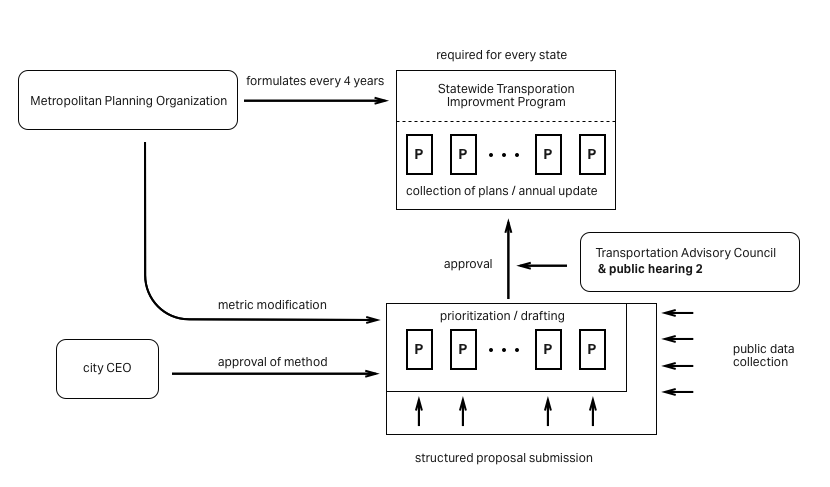
\includegraphics[width=\textwidth]{chapters/1/fig/proposed_process.png}               
  \repeatcaption{fig:proposed}{proposed method}
\end{figure*}

Other process such as Cambridge Participatory Budgeting project is capable of assigning budget to road infrastructure improvements. The current method provides a way to submit an idea to any given point of the city. The ideas are based on subjective comments and no cost estimation is there, with no data to support the claim.
Figure \ref{fig:proposed} shows the alternative method using bikebump. The main difference compared to the present standard procedure is; 1. Has a data collection method 2. Individual planning will be though the system, 3. City chief elected officer and the planning organization will commit by approving the system and modifying the metrics to meet with longer term goals that should be consistent to previous settlements and plans.


\clearpage

%steps for planning "community engagement"
%Determine the goals of the plan improve bike lane security
%not just reactive, but to start predicting potential threats
%Plan out who to engage
%bike advocacy groups
%Develop engagement strategies for the those individuals you already know
%bike advocacy groups
%Develop engagement strategies of those individuals you do not already know
%general community, including people using different
%Prioritize those activities
%Create an implementation plan
%Monitor your process
%Maintain those relationships

\section{Implementation Overview}

% The browser provide functionalities to record and process 
% 
% short description on the technological implementation
% web application, (client and server)
% few technologies used for bike bump
% The bikebump web application leverages various Web API's offered by browser programs
% Other libraries, but most notably React framework
% current web development are rapidly changing, javascript itself is a highly collective, programming language.
% Server
% for database, NoSQL Service based firebase offered by Google.
% [Diagram showing implementation]

This section goes through the implementation and techniques used for developing the application. The application is based on modern browsers, which recently extends the capabilities that were limited to mainly text and images. The WebRTC (Real Time Communication) is a series of protocols and APIs specifically for capturing audio and images and use them as inputs without plugins. The bike bump app leverages this technology to capture sound data. FFT will be applied to use get the frequency distribution of the called Web Audio API, 

Appendix XXX provides the extensive list of used APIs for developing the application.

The application is structured in form of a web application, which
components are the database, back end server, front end client. The database is a NoSQL, which stores data as a giant JSON data. To reduce the number of requests and efficient data transfer, the database contains some redundancy in memory.

\subsection{Definition}

The following is the definition for certain element that consist in the app.
% TODO: add image

\textbf{DING}

A DING is a spatial representation of a ring bell report. It defines the
geofence of the ding, with a center geolocation and radius. It also hold
information for each report which is the timestamp, users id and the
``good''/``bad value based on the study protocol. If there is a road near by the center location, it will also contain the roads identifier and distance from the closest point of that road.

\textbf{ROAD}

A ROAD is a geometrical feature that is returned by the Vector map API call. (Appendix. XX Vector Maps). A newly created ding will find the closest road registered in the Openstreetmap database and geometrical features will be copied to the bike bump database. When creating a improvement plan, users will first need to choose which road to apply an intervention.

\textbf{COMMUTE}

A COMMUTE is series of GPS location data, to know whole path of each ride session. Raw GPS data has tendency to bounce and contain noise, so it will be processed to match the road network in Openstreetmaps. Appendix XX shows which method was taken for getting the estimated path.

\textbf{BIKE COINS}

BIKE COINS are the currency for deciding which intervention to
prioritize. Each users will initially receive 100 BIKE COINS, which can be
distributed by the users choice.

\textbf{IMPROVEMENT PLAN}

A IMPROVEMENT PLAN is a combination of a CONTEXT and a SOLUTION.This
method of having a separate list of where (CONTEXT) and what (SOLUTION) and
combining them is taken from Christopher Alexander`s methodology of ``The
Pattern Language.''
\cite{alexander1977pattern}

The method of defining patterns (a recipe what to do in order to come up
with in outcome) and apply them to common cases is widely used in the realm
of software engineering as design patterns.
\footnote{although Alexander himself claims that ``design patterns'' in
  software is different to what he had create, since the patterns are distinctive, having no
interrelation between them.\url{https://www.youtube.com/watch?v=98LdFA-_zfA}}

Each IMPROVEMENT PLAN holds information of how many BIKE COINS it requires
to be counted as a community approved plan. This number can be calculated
using the SOLUTION`s type and unit cost, multiplied by the length of the
road.

\textbf{SOLUTION}

This is the execution instructions for a possible plan, such examples are
creating Bike Boxes and painting the lane with green paint.
This is separate from the CONTEXT focusing on only what to do for a
road, equivalent as the patterns in the Pattern Language.
Information that is included in one solution is name, description, type and
unit cost. The type is used to differentiate the solution needs to account
the length of the improvement or not. For example, a bike box will only be
needed for one intersection, where painting a lane in green will differ
with the total length. The unit cost is how much BIKE COINS would be
necessary per unit which is defined by the type. The unit cost will be
connected to the cost of the intervention. The cost will include but will
not limit to monetary cost, since some solutions will be
politically difficult even in relatively cheap interventions. 

For the experiment, three solutions where provided (Table \ref{tab:solution}).

\begin{table}
  \centering
  \begin{tabular}{|c|c|c|}
    SOLUTION & type & unit cost (m) \\ \midrule
    Green Paint & road & 25\\ 
    Bike Box & intersection & 320\\ 
    Plastinc Polls & road & 75 \\ 
  \end{tabular}
  \caption[solutions]{Solutions provided for Experiments.
    Values are estimated by material cost. Dimensions are taken from the
    Urban Bikeway Design Guide\cite{national2014urban}. Green Paint is
    \[5ft (W) * 2 (both sides)\] 
    BikeBox is
    \[12ft (W) * 16ft (H) \]

    Cost estimation can be done here 
    \url{http://www.asphaltkingdom.com/parking-lot-paint-calculator}

    Plastic polls are put in 2m pitch with each costing \$150
    \cite{aarian2016want}, therefore
    \$75 for each meter. 
  }
  \label{tab:solution}
\end{table}
\\

\textbf{CONTEXT}

The CONTEXT is a segment of a road which a Solution will be applied. The
system enables the users to select which part of a road they would like to
improve. The segment will include information of the length to by
multiplied to the unit solution cost if applicable.

% The browser provide functionalities to record and process 
%
% short description on the technological implementation
% web application, (client and server)
% few technologies used for bike bump
% The bikebump web application leverages various Web API's offered by browser programs
% Other libraries, but most notably React framework
% current web development are rapidly changing, javascript itself is a highly collective, programming language.
% Server
% for database, NoSQL Service based firebase offered by Google.
% [Diagram showing implementation].
\section{Interface}

The app has five major views; the recording view, the map view, the
vote view, the improvement list view, and improvement creation view. The
top navigation bar guides the user to jump between the views.

\subsection{Record view}

\begin{figure}[!htb]
  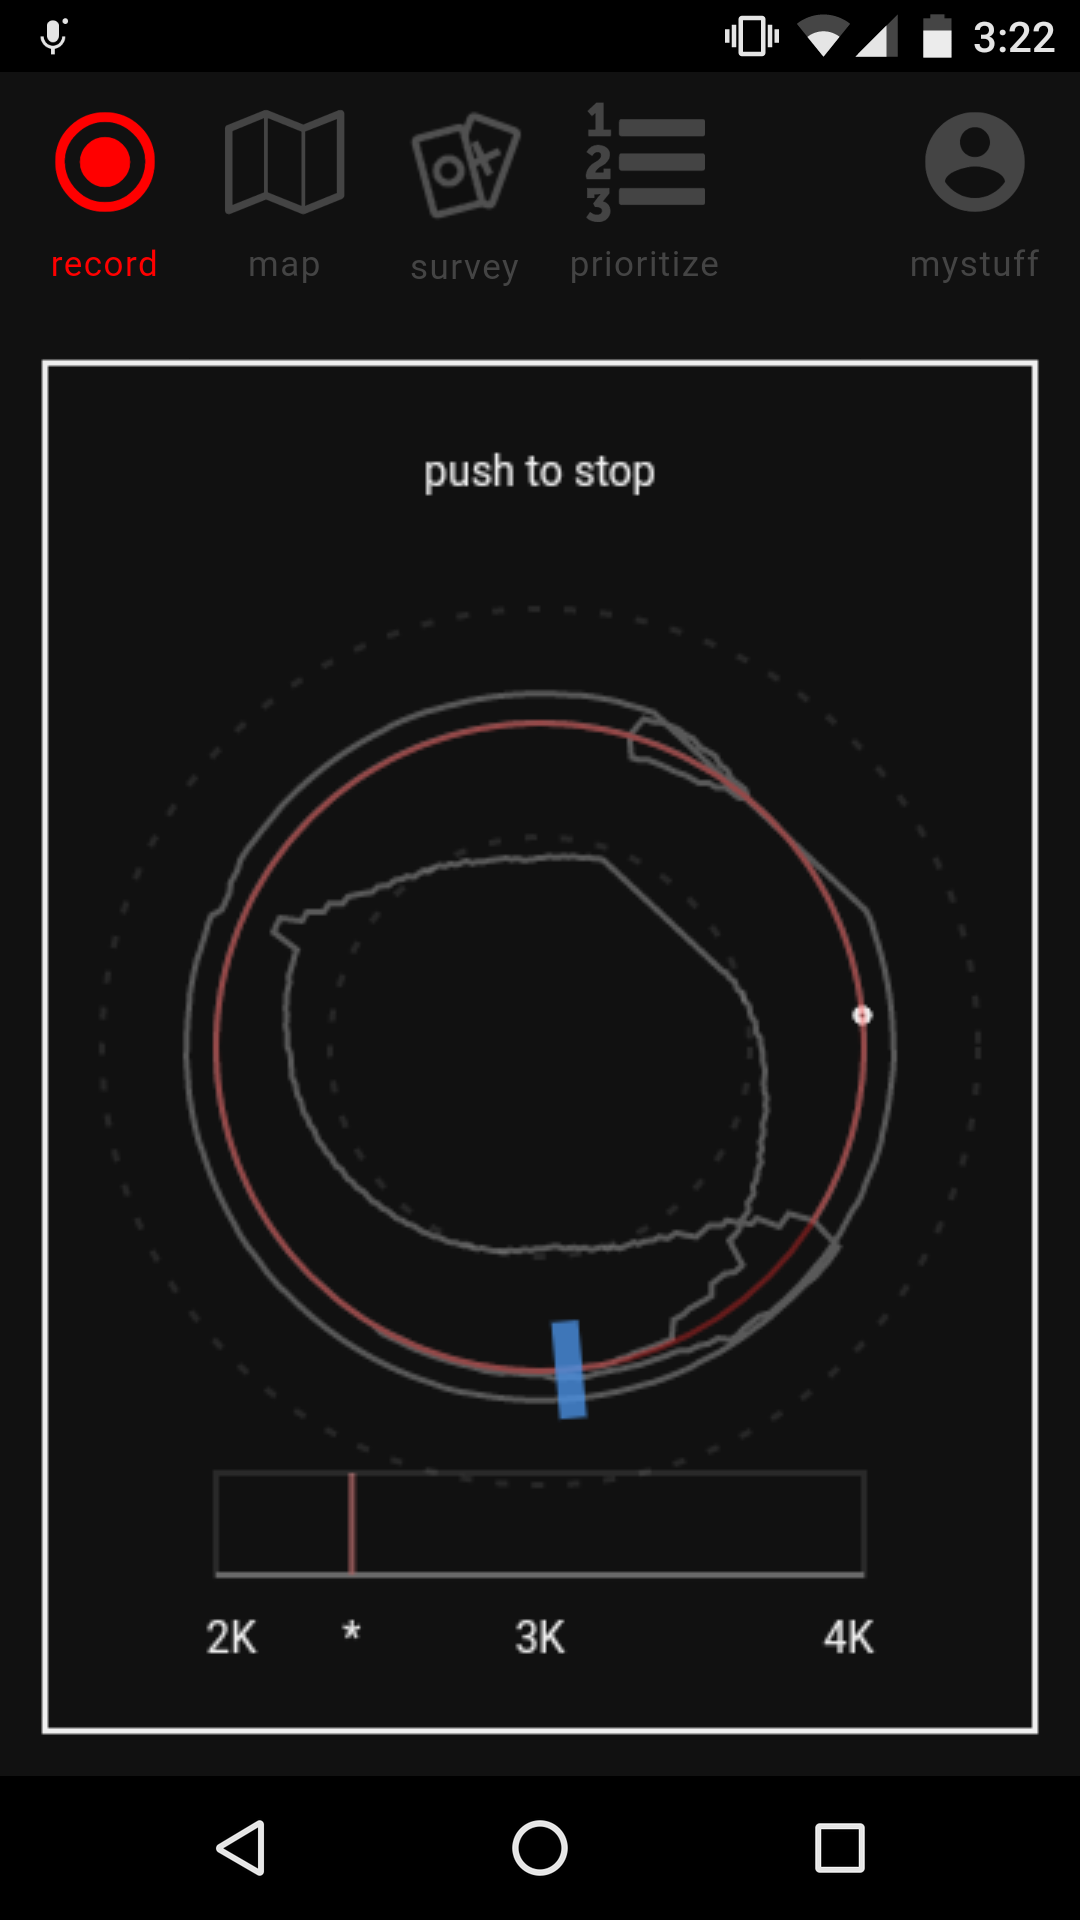
\includegraphics[width=0.6\textwidth]{chapters/4/fig/interface_recording.png}
  \caption[interface: Record]{recording view}
  \label{fig:interface_record}
\end{figure}

Figure\ref{fig:interface_record} is the main view when users ride their bike and
record the events. The primary function is to detect the user's bike's ring
and send it to the server. Based on given data from the calibration, the
application looks into the target frequency and validates two thresholds;
the slope through the adjacent frequency values and the duration that slop
threshold persisted (time limit).
Refer to\ref{appendix:time} for details on the method of ring bell detection.
The initial detection will store two things in memory; 1. The latest
geolocation and 2. A sound of 4 seconds before the detection.
\footnote{the recorder holds a data array with constant length and stores
  each sound input, overwrites the data each time it is full. This data array
  will be developed when saving as an audio clip. To exclude the first part
  of the detection, the system will record from -5 seconds to -1 seconds
relative to the detection.}
If once detected and  detected more than once in the succeeding 4 seconds,
the place is judged to be ``good,'' and if it is never detected, it is
judged to be ``bad.'' After the four seconds, the app will submit the
geolocation of the first location, sound data and ``good''/``bad'' label to the server, and returns to the initial state.
The users will be notified about this one ring is ``bad'' and twice means
``bad'' protocol before hand.

The interface uses animation frame to show the detection and the label data
``good'' or ``bad,'' with a circle orbiting the 4-second detection interval.
For safety reasons, when recording, other buttons are disabled to prevent
user input. Also while recording, the app will periodically query the
geolocation and store ``bread crumbs'' of geolocation.

\subsection{Map View}

\begin{figure}[htb]
  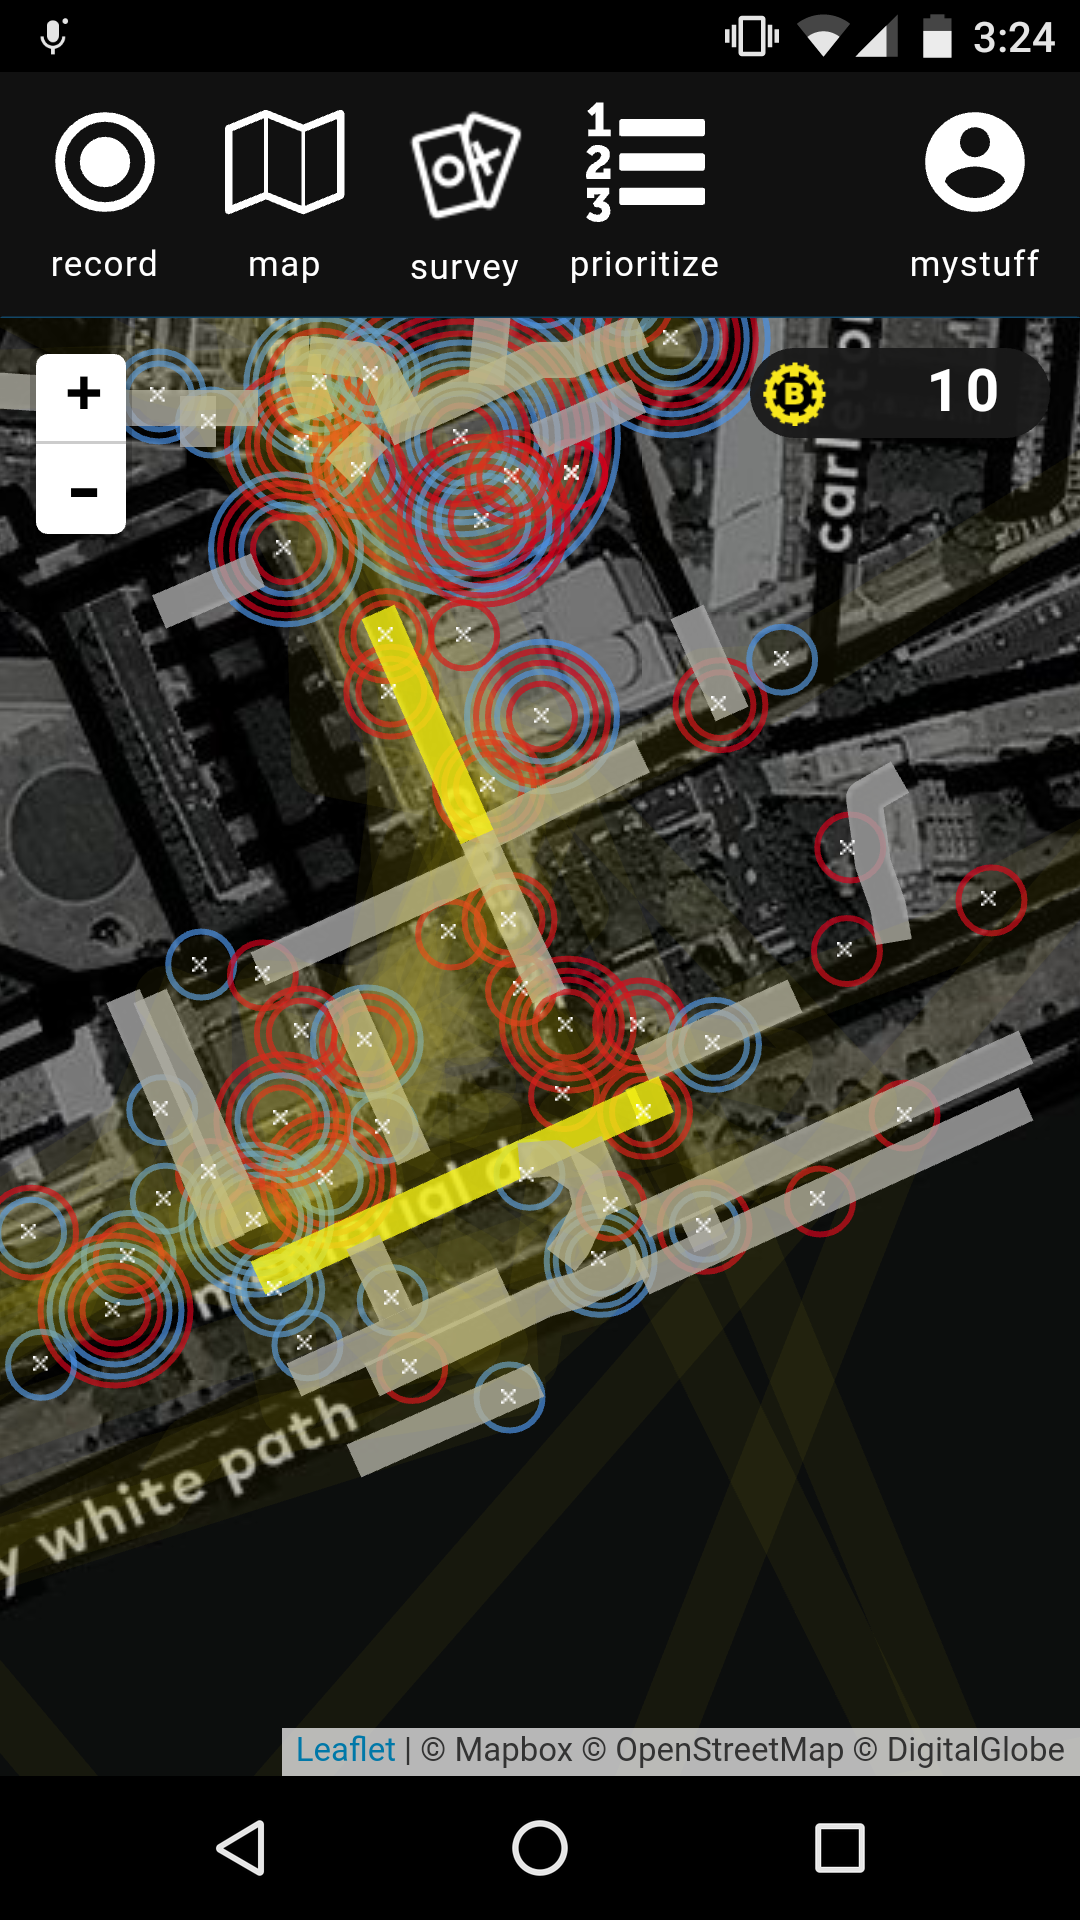
\includegraphics[width=0.6\textwidth]{chapters/4/fig/interface_map.png}               
  \caption[interface: Map]{Map view}
  \label{fig:interface_map}
\end{figure}

\begin{marginfigure}[{0cm}]
  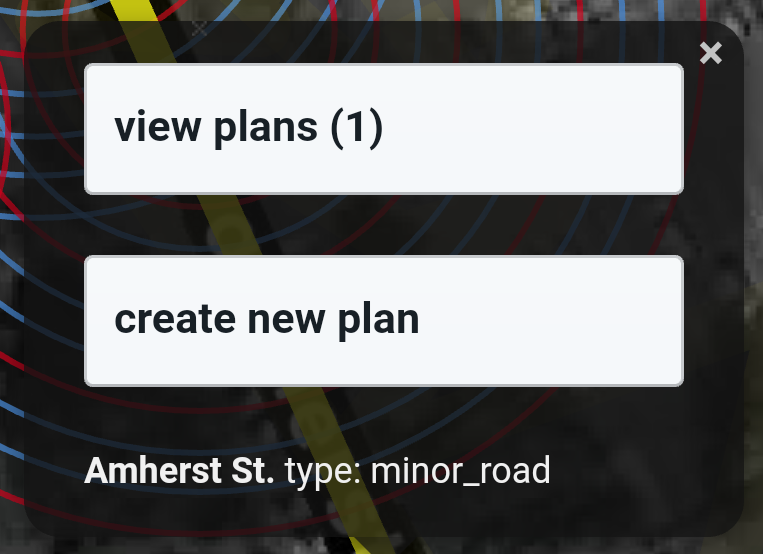
\includegraphics{chapters/4/fig/interface_popup.png}               
  \caption[interface: Popup]{a pop-up navigator linked to creating or
  voting to IMPROVEMENT PLANS}
  \label{fig:interface_popup}
\end{marginfigure}

The Map view (Figure \ref{fig:interface_map}) visualizes the data obtained by users.
The visualization includes geolocation data of people's DINGs, highlighted
roads that had one or more closest dings. The commute paths that people
took. Yellow road segments indicate that there was at least one improvement
plan submitted by any user. The roads have pop-ups (Figure\ref{fig:interface_popup}) that link to options to
existing improvement plans or the improvement creation view.




% The application was implemented as a smartphone interface
% Detecting locations that are unsafe
% detecting ring bells
% FFT performed by the microphone
% Attempt to catch specific frequency preconfigured by the setting.
% [image: bell]
% [image: interface]
% Query current condition to identify bike lane security
% Ask (mostly) binary questions to set the current
% Two reasons to ask
% have fine grain information on current situation
% ask users for current
% [image: interface]
% Visualise acquired report data
% mapping of unsafe areas
% [image: map plot]
% Solution Picking
% Solicit solutions by selecting from possible diagrammatic solutions
% Prioritisation

\subsection{Survey View}

\begin{figure}[htb]
  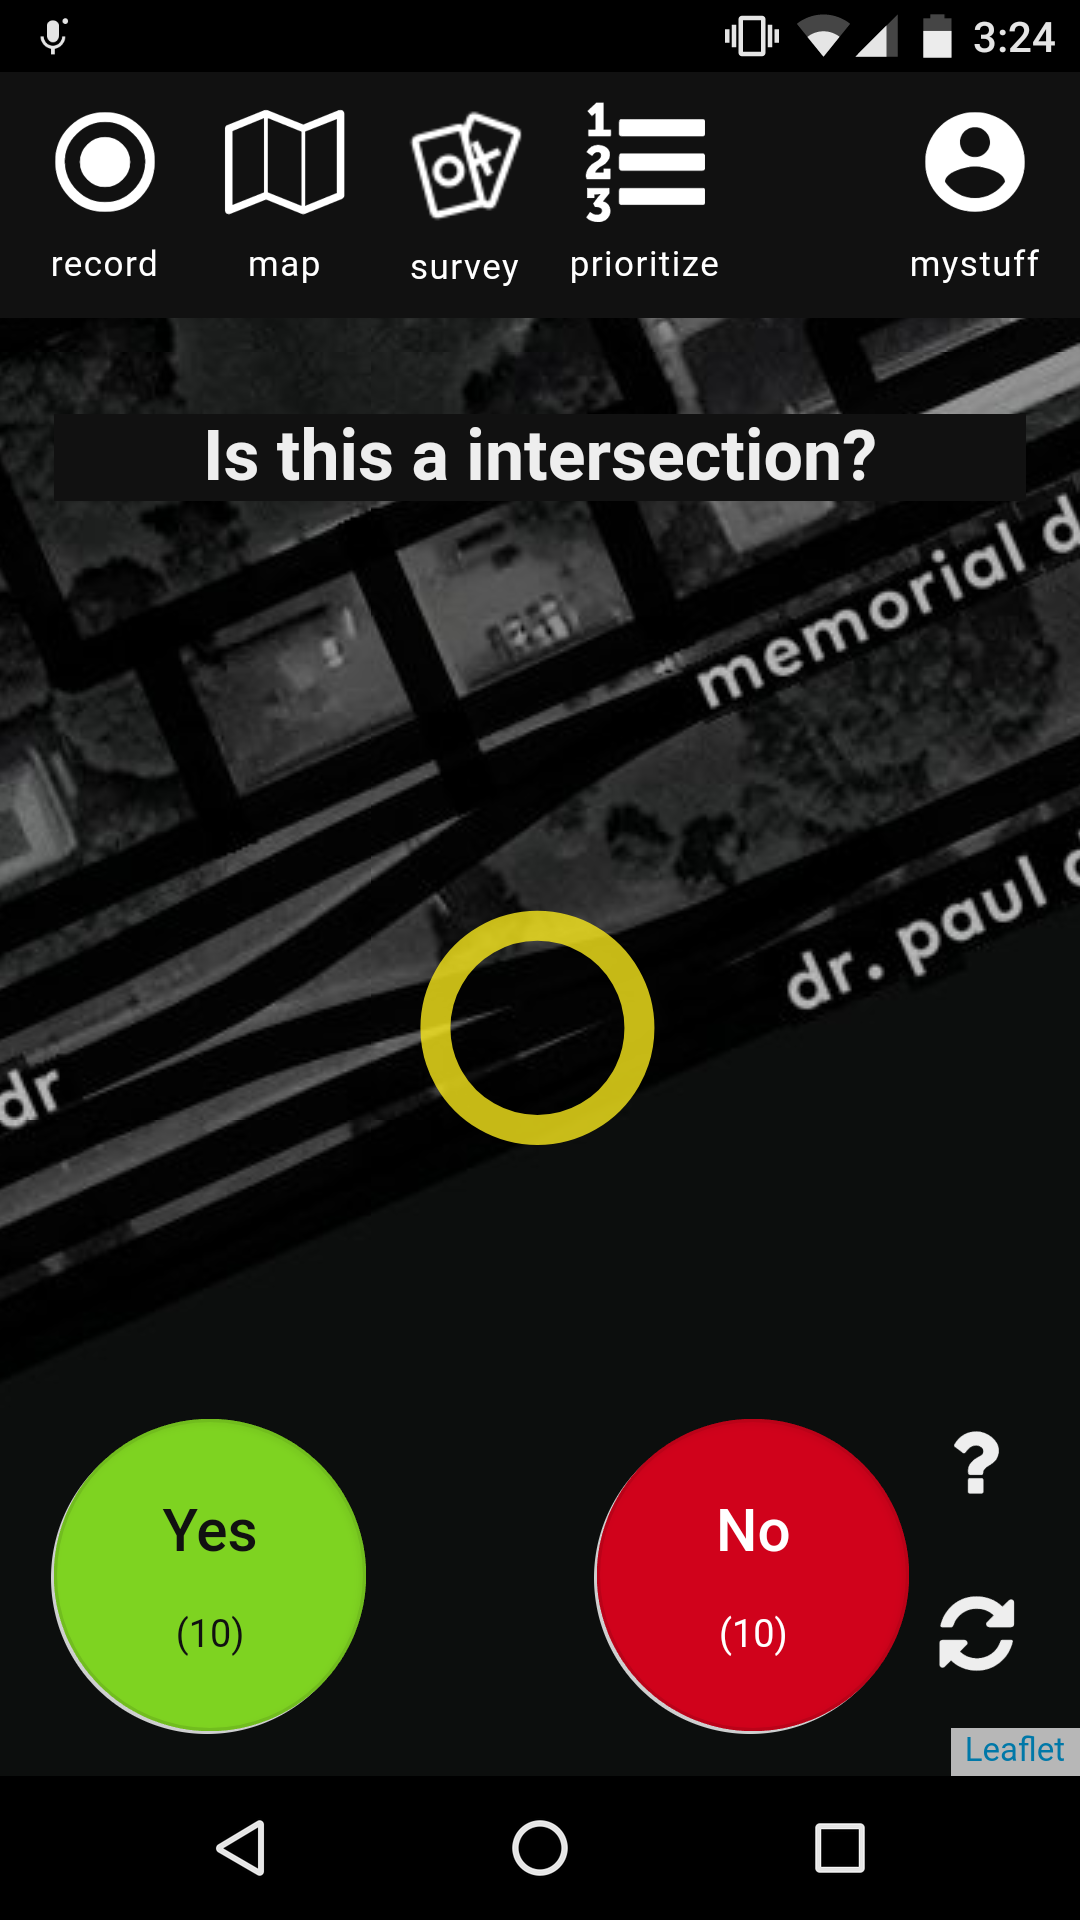
\includegraphics[width=0.6\textwidth]{chapters/4/fig/interface_survey.png}               
  \caption[interface: Survey]{Survey view}
  \label{fig:interface_survey}
\end{figure}

The survey view asks the users follow up questions to complement their ding
reporting. There are two purposes for having this feature, thus two kinds
of questions. The first purpose is to collect information that does not
exist in the Map Data such as OpenStreetMap (OSM). OSM data does not
include information about specific conditions about the bike lane, for
example, painted in green, or separated with plastic bollards.
\footnote{some Path network includes information on the existence of a bike
  lane or an attribute indicating it is a cycle path yet the data have no
guarantee that it is updated timely.} 
The type of questions that serve this purpose is for retrieving information
on the current condition. For the experiment, these questions were:

\begin{enumerate}
  \item Is this place an intersection?
  \item Was there a separated bike lane?
\end{enumerate}

Secondly, the reason for the ``Good'' / ``Bad'' judgments varies,
so requires more information to ask for specific questions why the
report occurred.
One ``Bad'' DING may mean bad because of a pothole or a car blocking the
bike lane (occasional conditions) or no bike lane (planning conditions)

\begin{enumerate}
  \item The road was bumpy.
  \item It had lots of three shades.
\end{enumerate}

\subsection{Create Improvement View}

The create improvement enables users to submit improvements to the system
to be voted by other users.
The pop-up menu that each road shows (Figure \ref{fig:interface_popup})
provide links to this view (Figure \ref{fig:interface_improvment}).
To create an IMPROVEMENT PLAN, it is required to select the SOLUTION, and if
applicable, which range to apply for the selected road. While editing, the
total BIKE COIN changes that needed for community approval. The user who
proposes any plan will need to decide the tradeoff between different
solutions and ranges.

\begin{figure}[!htb]
  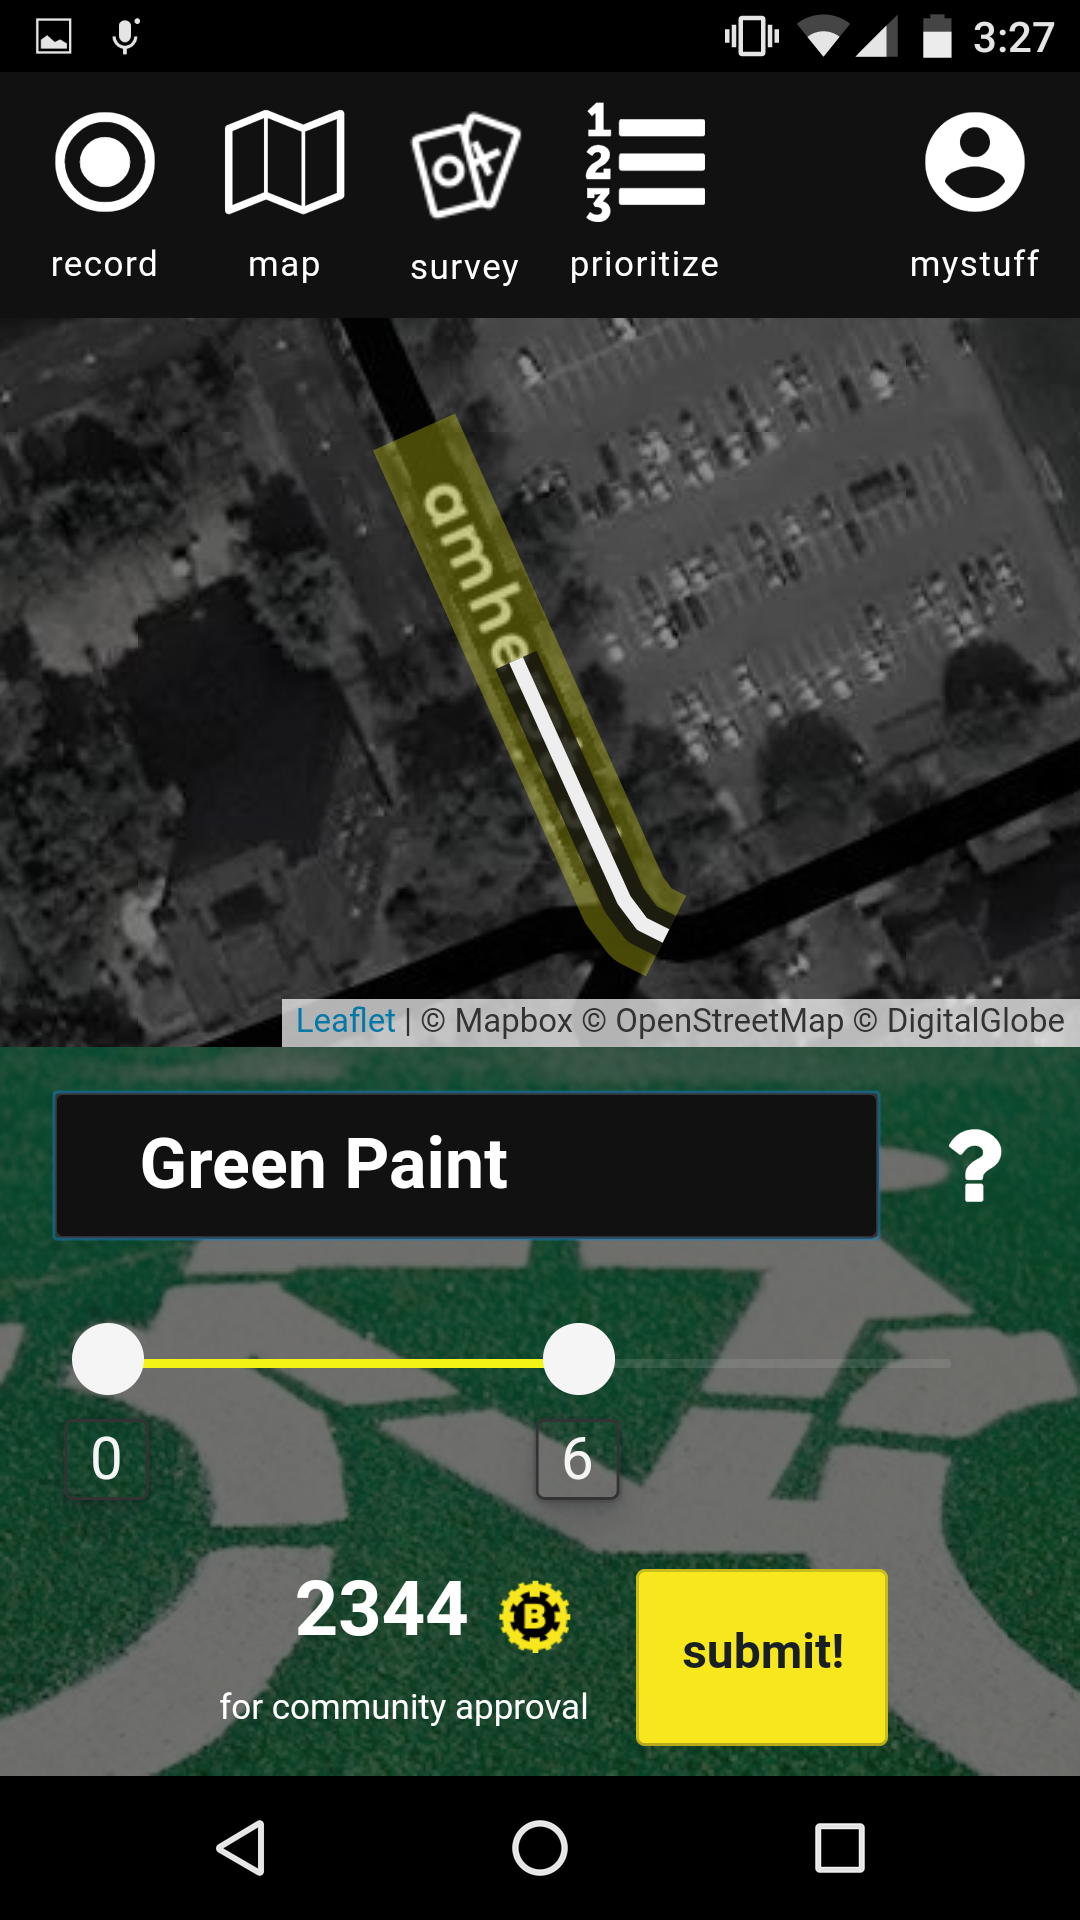
\includegraphics[width=0.6\textwidth]{chapters/4/fig/interface_solution2.png}               
  \caption[interface: Survey]{Survey view}
  \label{fig:interface_improvment}
\end{figure}

\subsection{Vote View}

Each IMPROVEMENT PLAN will have a VOTE view. It provides the interface to
distribute points for the segment. It is a four choice question, with the
option to give 0, 10, 20, and 50 BIKE COINS to the target plan. The app
permits the user to vote for their IMPROVEMENT PLANS created by themselves.

\begin{marginfigure}
  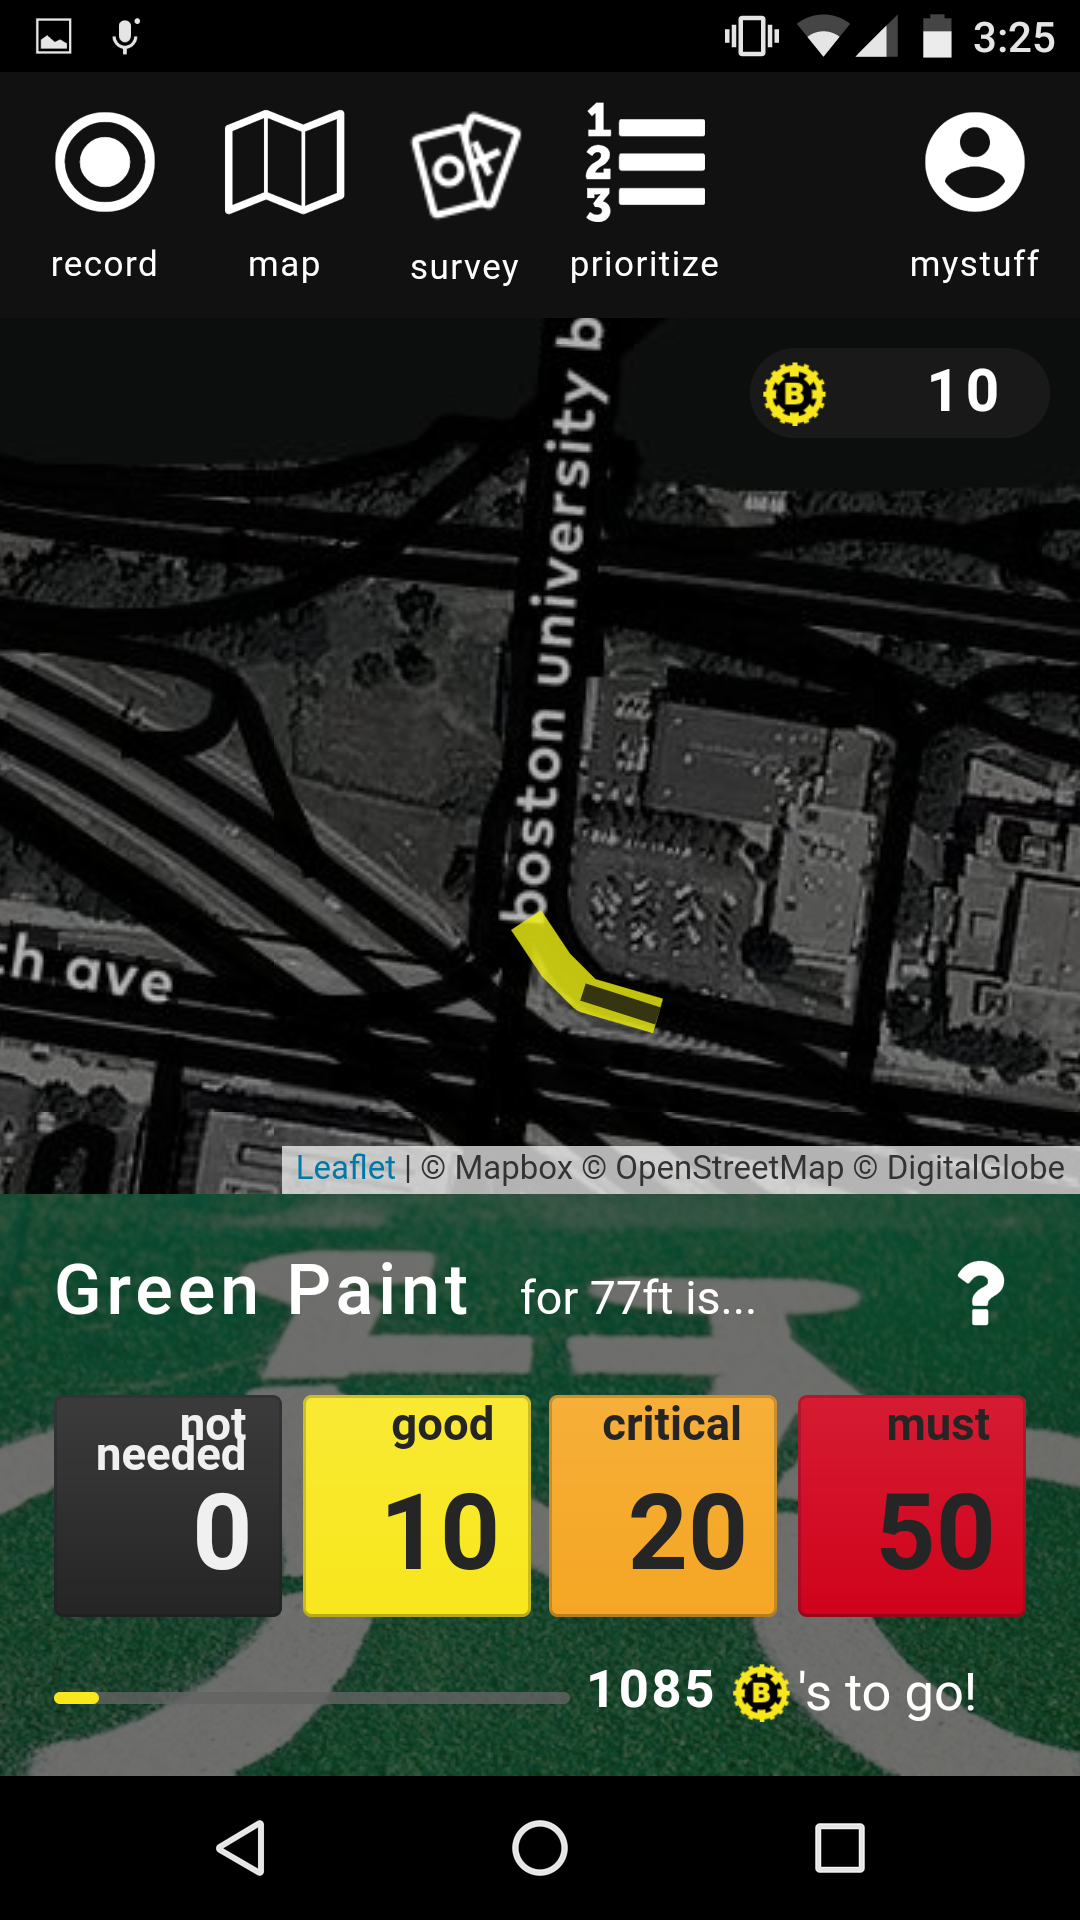
\includegraphics[width=0.6\textwidth]{chapters/4/fig/interface_vote.png}               
  \caption[interface: Vote]{Vote view}
  \label{fig:interface_vote}
\end{marginfigure}

\subsection{Improvement List View}

\begin{figure}[!htb]
  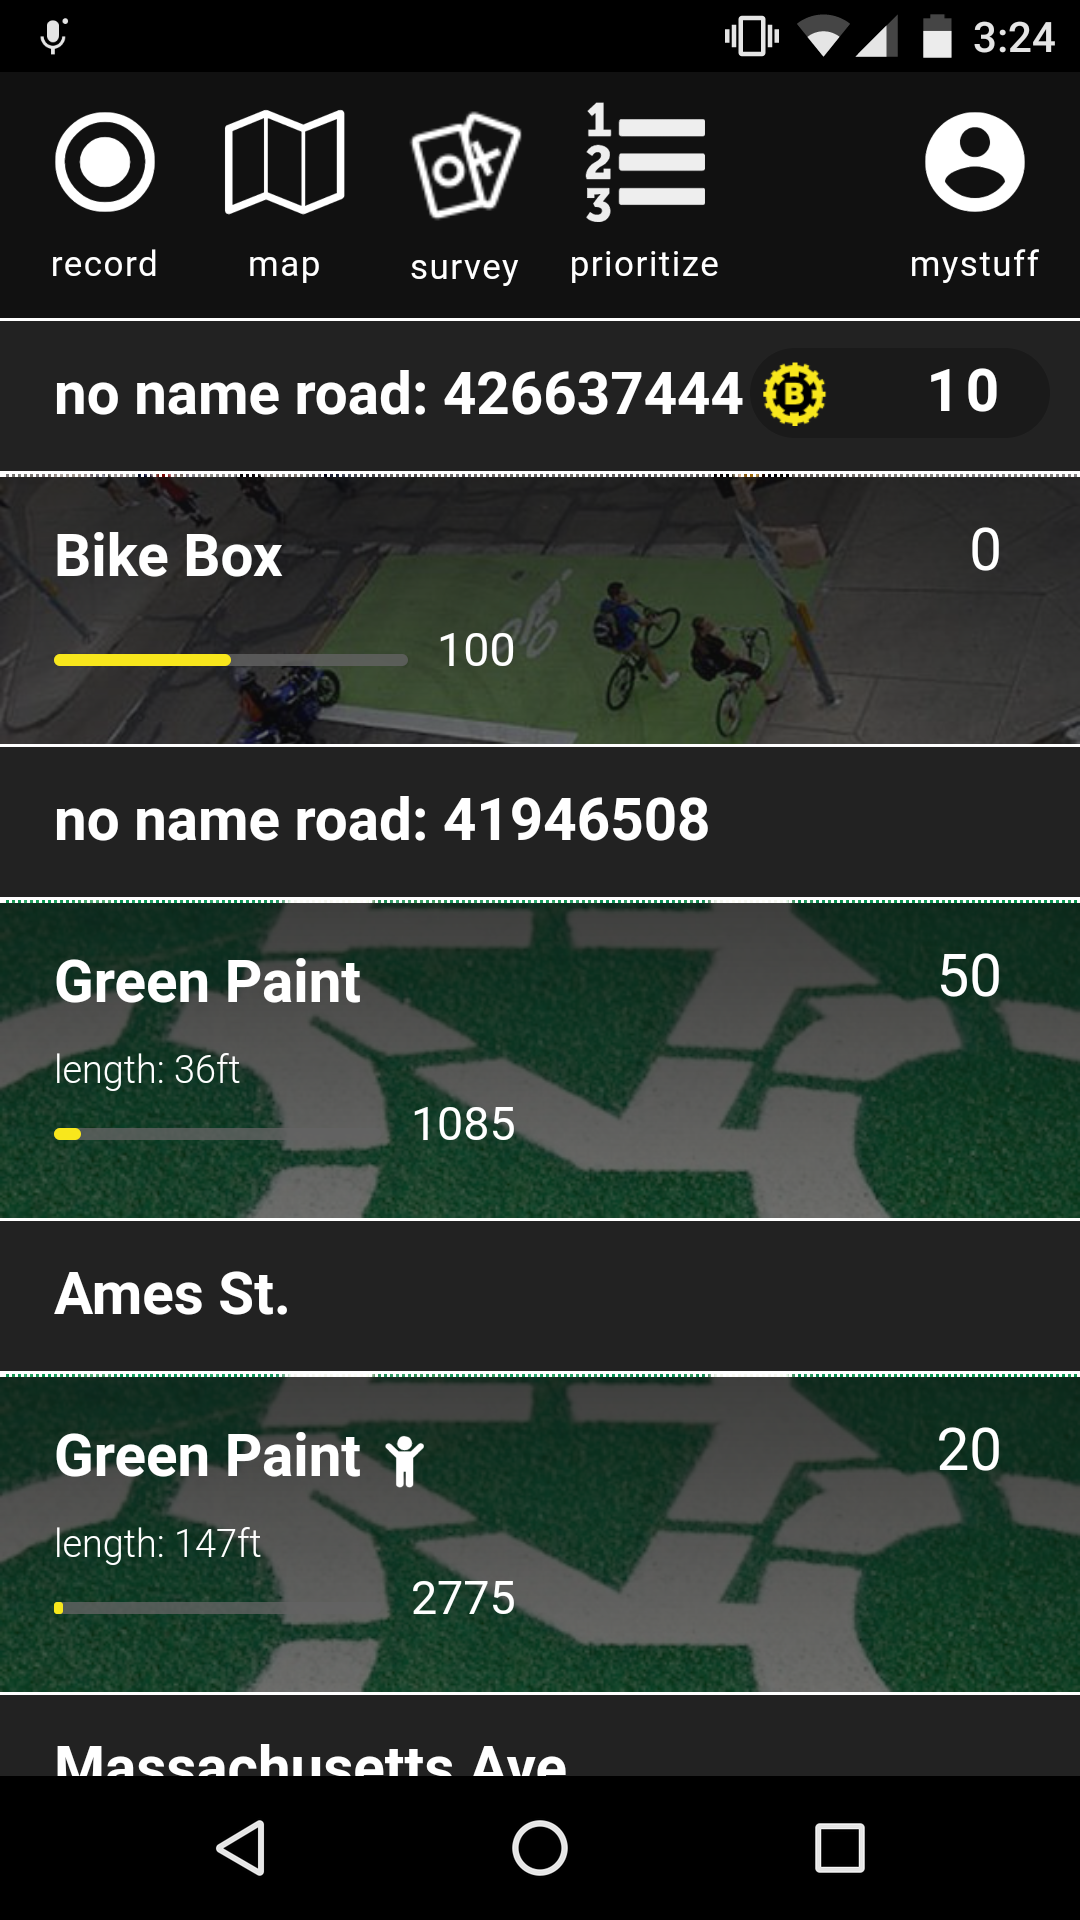
\includegraphics[width=0.6\textwidth]{chapters/4/fig/interface_list.png}               
  \caption[interface: Improvement list]{Improvement list}
  \label{fig:interface_list}
\end{figure}

The Improvement list is the where users can see a sorted list of each
improvement.
This list is sorted by the total number of BIKE COINS.

\section{Experiment Setting}

A human subject test was conducted to examine the functionality
and effectiveness of the prototype. Refer to Appendix \ref{app:COUHES} for
the complete consent form.

A total of 20 people had been recruited by email and social media posts;
the users demographic was students and individuals from local bike advocacy
groups. Out of the 20 participants, five were female subjects. Each test
had one participant.

Three participated using a bike sharing service\footnote{Hubway
\url{https://www.thehubway.com/}} others used their bike. 12 people used
the bell provided, and none owned a smartphone mount. The experiment was
conducted during the day, without rain, time slots were 9:30, 12:00, 14:00,
15:00.

Each test took around 1.5 hours. The experiment had four steps. The first
was the orientation, where the examiner introduces the objective of the
user test, gains subject's consent, asks for the initial survey, shows how
the application works, and talk about the route of the on bike experiment.

The second step is to have the users ride the bike, with the app running.
Figure \ref{fig: route} is the path that was asked for subjects to take.
The start location was the entrance of MIT Media Lab heading towards the
Charles river turning right taking the Dr. Paul Dudley White Path. This
path was renewed in 2017, with a bi-directional cycle path which is rare in
Cambridge. The route makes a left turn to take the Harvard Bridge, which
does not have a dedicated bike lane. Car traffic is relatively high since
there is no light until the end of the bridge. The intersection of Havard
Bridge and Beacon Street is infamous having accidents and considered one of
the most dangerous crossings. 
\footnote{a cyclist died hit by a tractor trailer in 2015
\url{https://www.bostonglobe.com/metro/2015/08/07/woman-bicyclist-injured-apparent-collision-with-vehicle-back-bay/zsjWYLZIZ324kSkmbjOaWM/story.html}}
In response to the number of accidents, the city of Boston has had modified
the lane structure for the crossing and Beacon Street. Proceeding to Beacon
Street, the route takes a slight right for Bay State Road. Park Driveway
crosses Beacon Street close to this intersection, which is also close to
the intersection of a major cross down Parkway, Storrow Drive. Bay State
Road is a one-way road with less traffic but no bike lanes and an arch of
tall trees in both sides. The users are asked to take a survey using the
app at the intersection of Back Street. Taking a short left turn, it is
Common wealth Avenue which a wide multi lane road that is a part of an
arterial route. Despite the wide road and fast traffic, there is no
separated bike lane. Subjects take the BU Bridge heading back to Cambridge.
Over the weeks of experiments, this BU Bridge was shut down to cars
allowing only pedestrians and bikers to cross.
\footnote{Boston Globe reported the happy comments from the cyclists, right
  after the shutdown. \url{https://www.bostonglobe.com/metro/2017/07/28/for-cyclists-bridge-closure-like-heaven/bBWnlm00ROV7LfZW0w7f2O/story.html}}
The BU Bridge ends with a roundabout that does not have lights or separated
bike lanes. The route turns left after the roundabout to Waverly Street,
thin single lane street. The path turns right before the park to take
Vassar Street. Vassar Street has a dedicated bikeway at the same level of
the side walk. The route returns to the Mass Avenue crossing MIT's main
entrance. This part is often crowded with tourist buses with many
pedestrians crossing. It is also close to the bridge, which the drivers
rush to catch the light with high speed. Lastly, the route heads back to
the origin using the same path, but the different side.
There is a lengthy discussion on bikes riding on sidewalks, and the law is
different depending on the area. Massachusetts law permits bikers to use
the side walks if the local city permits to do so. 
\footnote{Massachusets General Laws PartI Title XIV Chapter 85 Section 11 B
\url{https://malegislature.gov/Laws/GeneralLaws/PartI/TitleXIV/Chapter85/Section11B}}
The city of Cambridge does not ban bicycles to use the side walks in
Memorial Drive. /footnote{Sidewalk Bicycling Banned Areas.
\url{http://www.cambridgema.gov/CDD/Transportation/gettingaroundcambridge/bybike/rulesoftheroad.aspx}}

This on-bike test was designed to take approximately 30 minutes. Within the
experiment, users were required to stop and take an in-experiment survey.

After the user had come back from the trial, a discussion was held to know
how people perceived the ride with this app.

% 
% summary of results, raw data will be attached to the Appendix
% mapping
% inputs from users
% technical results
% ring detection success rate
\section{Results}
\subsection{Quatative}
% have basic statistics of the amount of data collected through the experiment
\textbf{Accident report comparison}
70/% of the bike accident reports were included in at least one ``Bad'' DING.\footnote{a DING that the have larger amount of ``Bad'' reports}
% have basic statistics of the amount of data collected through the experiment
\textbf{Ambient sound noise and `bad' report correlation}
Sound clip data did not show (Yet!), ambient noise influences
    peoples perception of ``Good'' / ``Bad'' when biking.
\tectbf{BU Bridge before and after}
The tendency of the report changed radically after the bridge shut down.

\subsection{Quantative}
A summary of the replies for the after bike discussion follows the next section will discuss the subject's response in detail:
\start{itemize}
\item None of the people knew the standard process to change a road. 
\item Most of the people recognized that this could be useful to learn the collective opinion and maybe able to replace the current system without modification.
\item People said, ``Bad'' reports were often a moment or a point, where ``Good'' reports were often a continuous feeling.
  \item The majority of subject felt awkward when ringing the bell when there was someone in front.
\item Participants understood there are two distinct processes, and felt it is useful to have them integrated into one.
\item The interview has a section that discusses the two usages of the app. One is open access where the citizen can download and use when ever they wish, create improvement plans and vote for them without any limitation. The second possibility is the city concentrating to a specific road they think they need to improve and set predefined improvement plans 

    than being told by the city to concentrate on a particular route.
\end{itemize}
\section{Evaluation}
\subsection{Analytical side}
\begin{itemize}
  \item Most of the people said the app functioned as intended, while there
    were some complaints it was unstable when large vehicles (trucks and buses) passed.
  \item The analytical side showed that this method might be an indicator
    of accidents, yet it is important to know where people moved, since the
    data may be biased towards particular routes.
  \item It is hard and too early to say that both DING positions and sound
    clip data are a good predictor of bike accidents.
  \item Relativeness - There were multiple times people stated that they
    felt danger when the bike lane disappeared. Talking that safeness is
    relative to the previous feeling of being safe. This comment is an
    indication that already it is a wicked problem.
\end{itemize}

\subsection{Synthetic side}
\item It was rather obvious that none of the people knew how to propose an
  improvement plan. The trend was the same for the foreigner's regarding
  their own country.
\item Most people said there is no disadvantage having a proposal layer on
  top of the data layer. Some stated it is better to have the analytical
  side and synthetic side integrated since it is easy to go back and forth.
  While there were some opinions that the integration could be much more
  intuitive.
\item There are two ways to use this app in practice. A controlled
  engagement where the city provides the particular segment and for  the
  call for data collection and improvement plans. In contrast, a free
  platform that the citizens/participants are free to collect data and
  submit improvement plans to their demand. Most of the participants
  preferred the free version, yet lead to a dilemma that if it was free to
  use, there is very few chance to encounter that app or ever installing it
  and may be used and dominated by serious bikers, which is exclusive and
  opposite having a grassroots method.


% \chapter{5. Discussion}

This chapter discusses the implementation of the bikebump application and the
factors requiring consideration when creating a collective urban design tool
that effectively engages the community.

\section{A generalized tool for collective urban design}
We have been investigating a new tool for having a bottom up urban design method.
The bikebump application concentrated on having two basic elements of design,
each having two sections within them. These four elements will be the building blocks
of a mobile community engagement tool for collective urban designing.
The following will cover the design decisions that each component should consider.

\subsection{Analytic Phase}
The analytic phase is where the community learns the current situation in two dimensions. One is the individual level, where they experience the road themselves. Paying attention to the road condition changes the way they think while riding.
\footnote{18 out of 20 people said the application made the subject aware about the road condition.}
These individual experiences gather and compile into a collective view. Users can interpret the results relative to what they felt while riding. This aspect is different from when only the urban planning professionals draft the plan, often only looking at the visualization.

\textbf{1. data collection} \\
Bikebump used the DINGs as a method to collect data. As an urban design tool retrieving the geolocation data from devices will be mandatory. Deciding what other data to collect changes how much
we count on the humans as sensors. We could make the decision to record the sound of the whole commute and process it afterwards. This relies more on the sensors themselves and the assumption of what kind of sound people think is dangerous. Methods that fall in the same category vary in what kind and how much rich information we collect.

The application might record accelerometer data to detect places where people suddenly change speed, or take a video to later process to image recognition techniques. The other aspect is the human sensor, which for bikebump was the act of people ringing the bell for reports. The experiment explicitly did not specify the definition of ``good''/``bad'' except mentioning this was an attempt to improve bike lane security. \footnote{This is a design decision whether the experiment focuses on human perception, which is often ambiguous signals different from exact readings from mechanical sensors.}
Alternative to this approach a simple button to collect the perception.
\footnote{Within in the iteration of development button input was considered, but has been rejected for two reasons. One, it was dangerous to have people interact with their phones when they think it is already dangerous, thus having biased data. Very few people ride their bikes with bare hands in winter.}

The black box may remain a black box whether we combine the sensor data and try to correlate the two methods of data acquisition, but advances on extended intelligence\cite{pubpub:extended} may lead to accurate predictions of people's perceptions. The difficulty of this is the human sensors adjust to the environment and previous experiences. Cities with a lot of safe bike lanes may be very sensitive to small issues, relative to places that do not have much bike safety infrastructure. Not only that the app itself may change the behavior of reporting, after knowing the synthetic phase, people will digest the experience and adjust the definition of ``good''/``bad''.

\textbf{2. visualization} \\
The visualization was what the subjects observed after different kinds of data were processed. The main difference between other visualizations is the purpose. Attempts that end as a visualization is to give the observer an insight of a what the data shows. In addition to this, the visualization for a collective design tool should bridge the synthetic phase and what people have proposed. This means at least two different types of information will be superimposed: the result of the data collection phase and what was proposed to improve the place.

Bikebump visualized the consecutive GPS readings throughout the commute to show where people have actually passed. This will be a mechanism for balancing the improvement plans, since the number of DING reports may not always align to the trips taken.


\subsection{Synthetic Phase}
The RVSP cycle is a design process that is not constrained by the order of each R, V, S, and P phase. Alexander clearly mentioned the order of the analytic phase coming first.


One remark from the user test was the application is too organized toward being a linear process, which the user may not always follow. The application does not force the process to be completely linear, 
\footnote{There was a constrain of the order for proposing. An improvement plan was only able to be created if the ROAD had at least one DING report associated.}
\hlcyan{but the accessibility of these functions\footnote{report, view map, propose, vote} could have been weighted according to the usage frequency of an average user.} The application did not take this into account and it remains an open question, since the objective of each user may differ, and may change each time. Consequently, this may be one reason this kind of collective urban planning tool should remain separate from the analytic phase and the synthetic phase. Yet there is still the possibility that without the analytic phase, the synthesis phase would be biased towards subjective preferences.

Compared to various analytic phases that show visualizations and provide understanding, a structured synthetic phase has not been around. People may not be aware of the reason; thus, additional incentives may need to be considered, covered in p.\pageref{sec:incent}

\textbf{3. solution creation} \\ 
This section is the most mentally demanding section of the application. \hlcyan{It suggests the main findings was the reality that subjects doubted that their actions would have a real-world effect. They did not know how start interaction in the first place.} In addition, the interface tends to be the most complicated because the amount of information it handles is large. In bikebump, the users had to look for the road and its region, and match the specific SOLUTION type. This section could be more constrained, limiting the possible solutions, for example, to only one solution.\footnote{Ex. Just painting the road.}
\hlcyan{The key factor to show that their input will influence the process is outside of the design of the application, but rather building social norm that the application will make changes.}

\textbf{4. prioritization} \\
This phase can be interpreted as a collective sorting phase, where people use their own mind to order the improvement plans submitted by others. This phase is less demanding compared to the solution creation section, but the interface should be carefully structured, as this is where the judgment happens. Given the fact that this tool will always have geolocation, and sorting is the act of reordering the list, it is natural to have it plotted in a map and a list. In this case, the method for how the system sorts the list is an important factor to consider.

\subsection{How to tackle ``relative'' valuing}

One finding is the reports are ``relative'' to the previous experience. This is another characteristic of the `wicked problem', which `wicked problems' are essentially unique. \hlcyan{There may be overlapping contexts for each situation, yet does not guarantee that a single difference overrides the importance and influence the decision. The intersection where Beacon street changes to Bay State Rd, was showing the relativity of the timing of intervention and the location. The experiment was after the upgrade of beacon street, which is different thinking an intervention without that improvement, similarly it deforms the issue knowing that there is a safe road before that and the gap is the dominant aspect in consideration.}
\cite{rittel1973dilemmas}
It is unique since each user may have different perceptions on bike lane security, but more importantly, it is relative to the previous set environment.

Multiple people commented on the relativity of their perception. Data shows they felt insecure when bike lanes disappeared,
\footnote{The intersection of Beacon Street and Bay State Street, which the separated bike lane disappears. This separated bike lane was installed in response to a bike accident.}
\hlcyan{Despite this perception of unsafety, we do not know whether overall safety has actually decreased}

The users’ feedback also cast new questions on how to annotate the city. Bikebump used a 15m radius geofence as a method, but users implied that ``good'' situations were likely to be a continuous experience rather than a moment reaction. Measuring methods looking at a constant input may also validate this perception

\section{Incentives for bottom Up design, do we care?}
\label{sec:incent}

It is likely that bikers are aware that the city is still dangerous and needs improvements. Yet none of the subjects know the interventions the city is contemplating.

One reason may be that the mental threshold of changing their city is so costly that they do not even bother learning how to inspire the city to make changes or \hlcyan{may be that these procedures are bureaucratic and opaque and hard for people to acknowledge}.

This might be supported by the fact that younger people tend to moving more frequently, which whether you devote for any participatory design, you will be living somewhere else by the time you are able to appreciate the physical change.
\footnote{It is apparent that younger people move more than the elder generations. 
\url{https://fivethirtyeight.com/datalab/how-many-times-the-average-person-moves/}
, yet there are reports that the rate of younger people moving is decreasing over time.\\
\url{http://www.nytimes.com/2012/03/11/opinion/sunday/the-go-nowhere-generation.html}
}

Shorter span reward is preferable, and it may be preferable for different reasons. We can see this by the
loop of dopamine coming from the instant gratification from peer approval on social media networks.

While this thesis stands on the fact that the application or website is already recognized by the user,
it is important to consider how to design the initial contact.

\subsection{Initial Contact with citizens}

\textbf{Where} \\ 
In the after-bike discussion, more than half of the people said that they preferred not to have the city supervising or the planning side set a concentration area for getting input. People demanded an open platform that they report, propose, and vote whenever and wherever they wanted. On the other hand, people also recognized that if that were the case, \hlcyan{the likelihood of overlapping events being registered by the app would be totally by chance}. This creates possibilities for how we recruit participants. It is easier to start from a trial that has a target path, meeting the need from the city, and to gradually expand to a greater audience. This is possible, because of the mobile characteristics of the application, and is unique compared to the traditional methods of community engagement.

\textbf{When} \\
Methods that require people to meet physically has a limit to the physical space but time is also a constrain. It is hard to coordinate these two and have the majority of the people building consensus. The application can be installed and used anytime, yet the capacity of human cognition in a given time is also limited. A survey shows that most of the Android applications lose 77\% of the daily active users after three days.
\footnote{\url{http://andrewchen.co/new-data-shows-why-losing-80-of-your-mobile-users-is-normal-and-that-the-best-apps-do-much-better/}}
It is also true that even in the cases of the most dreadful natural disasters, we easily lose interest in after a short period of time. 
\hlcyan{Figure {\ref{fig:tohoku_trend}} shows this trend, yet we can see that people recall the disaster every year which is an attempt to delay being forgotten.}

\begin{figure}[!htb]
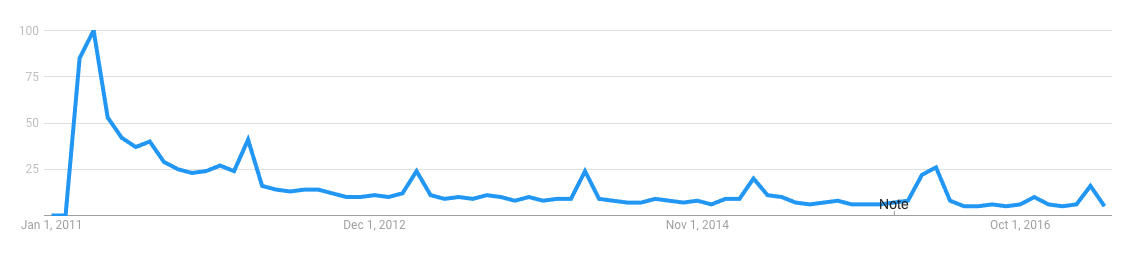
\includegraphics[width=\textwidth]{chapters/5/fig/tohoku_trend.png}
\caption[Trend for North East Japan Tohoku Earthquake]{\textbf{Google Trend} number of searches for the term `North East Japan Tohoku Earthquake'. We see a sharp degrade after the disaster, but periodic pulses occurs every year maintaining attention.}
\label{fig:tohoku_trend}
\end{figure}

The proposed process to incorporate Bikebump in the current TIP method still has an annual cycle to update the list of demanding improvement proposals. 
Rather than releasing the application and waiting for the community to spontaneously participate, a periodic campaign may be effective.
If we think of the attention from the public as something we need to raise, a report from the Nonprofit Research Collaborative
\footnote{\url{https://npresearch.org/pdf/2014-reports/NRC_AnnualFund_SpecialReport_July_2014.pdf}}
also points out that nonprofit organizations tend to meet their fundraising goals from annual funds.

\subsection{Communal value to Civic value}
Shirky points out that the internet has lowered the threshold barrier to coordinating with each other,
and within this collective action,
there are two kinds of value mechanisms; communal and civic values. \cite{shirky2010cognitive}

Communal value is created and acknowledged by the same group. \hlcyan{On the other hand, civic values may be created by a small group but acknowledge by the whole society.} Although bikebump targets modification in
infrastructure, it is fundamentally by bikers that benefit the same group, which makes bikebump's engine the communal value behavior. \hlcyan{It is different from examples like Wikipedia, which the authors and editors of posts is substantially small compared to the group that benefits from their effort.}

One comment from the user test was the personalization of the application.
The application did not show identity.
\footnote{except distinguishing individual proposals.
One concern that users will be able to identify other users homes.} 
Waze uses icons to show other users in the map, aiming for the sense
of community within the people who drive in the same area.
Personalizing the application interface may make the user feel
more attached to the application, and emphasize the sense of a collective effort.

Allowing others using different modes of transportation is the next step for inclusion. For the analytical phase, \hlcyan{drivers and pedestrians could have an application that lets them give feedback on when they felt endangered, or had a close call with a bicyclists. By enabling small but all kinds of individuals participate, the civic value will increase.}

\section{Micro owning and share economy}

Focusing on bike lanes, bikebump was one utilization of
the collective urban planning tool. \hlcyan{Despite the existence and successful testing of this platform, it is impossible to extrapolate and conclude that this method will work for other aspects of urban infrastructure.} 
\footnote{For specific applications, refer to the future work (p.\pageref{sec:future}) section in chapter 6.} \hlcyan{To have this method applied to other urban planning issues, these applications may need to change the social norm of how we own the city.}

We see the traces of the commutes from the map visualization generated from the users.
Although this was initially added to see how the commutes were \hlcyan{concentrated},
we can have another perspective that this is the traces of micro possession.

From the popularity and rise of mobile phones, there is a particular group of services that have been emerging; share economy related services. These new mobile-dependent services
\footnote{Car ride share and bike share services are obvious, but also Airbnb does not let you book without
a smart phone, Android tablet, or an iPad.
\url{https://community.withairbnb.com/t5/Hosting/How-to-accept-reservations-via-cell-phone-but-wittd-p/11129}}
are anticipated to be disruptive innovations that especially make the cities’ resources efficient.

Yet urban areas have been a sharing space for a long time. Restaurants are shared places to eat food.
Parks are shared areas which cities maintain using tax income. Infrastructure like roads should be included as well.
The only difference is that the parks and infrastructure are publicly operated by the government, it is owned by no one but everyone.
In contrast, new shared economy services ``share'', meaning users temporarily claim partial ownership. Without the support of these mobile applications, it is too risky thus the administrative cost is too expensive to maintain a ride sharing services without peer monitoring. The services leverages the computation the crowd holds to distribute opportunities for each member. As a result the services enables people to coordinate, negotiate, and ensure fair and transparent business.

We can say that a person who rents a bike from a bike sharing service owns the bike within the ride, but in addition, he also owns a fraction of road infrastructure within that very short time, which he then has the right to claim that his route should be safe. This is certain that when accumulated, commute routes become more ``yours'' than a place you never visited.
\footnote{This may be also taken as micro adverse possession, while currently it is not allowed to claim possession on public areas. Rose claims that the origin of property is possession.\cite{rose1985possession} The one who communicates the claim should in fact be rewarded with the property, because the act of clarifying property is already useful labor, that prevents costly conflicts thus facilitating trade.} \hlcyan{This leads to urban design not constrained with district levels but multi layers of partial ownership overlapped. The basic right for using the road may still be guaranteed, but the right to change the infrastructure to better suit the need will depend on who uses the road. It will be only within a prediction what will happen if this method was implemented, but we can guess the governmental scale will shrink in dense cities, since the ownership will fall in to regions that people can walk. If we see from Lessig's perspective, we can see this as a shift to ``market'' from ``law'', where the currency used for this market is the total time it was used.\footnote{Although it remains hypothetical, using time as the currency is fundamentally equal to everyone.} We see a city that is formed organically without a central government system much like the rich landscapes that Rudofsky's exhibition ``Architecture without Architects''} \cite{rudofsky1964architecture} presented. \hlcyan{To practically test this concept, one way maybe using a similar mechanism to Estonia's E-residency program. This program lets people create, own and maintain businesses without physically being at Estonia. In this micro owning case, we need a virtual government to grant rights to people who claim a portion of the city. Once being a virtual resident, the possession recording app will collect locations that the user passed or stayed, calculating where and how much the user owns in a microscopic way.}



% %% This is an example first chapter.  You should put chapter/appendix that you
%% write into a separate file, and add a line \include{yourfilename} to
%% main.tex, where `yourfilename.tex' is the name of the chapter/appendix file.
%% You can process specific files by typing their names in at the 
%% \files=
%% prompt when you run the file main.tex through LaTeX.
\chapter{6. Conclusion}

\section{Future Work}
\subsection{a general platform to conduct participatory urban design.}
Current applications like citizens connect is a general purpose app limiting at reporting. 

While it will be useful to have a general app that goes beyond reporting but enables users to propose an intervention, there is a risk that it is hard to maintain the attention for one mobile app. An alternative is to create a framework of the app, which can be customized to specific targets similar to bike lane security and topics discussed in the DISCUSSION section.

Recent web application development have focused on modularising parts to make it easy to reuse and distribute. We can observe this by NPM (Node Package Manager; A software that automates dependency checking and installing parts of software to be used in combination.) Having more than 475,000\footnote{https://www.npmjs.com/} building blocks that one can combine to make web based applications. The elements of one application is modularising as well, were one application are components combined together.

\subsection{safer route navigation}
Utilizing the data collected by the users, we can make a routing system based on safeness within the roads.

Modern map services enables custom path finding, where applications can set different weights for each road segment. Improving the overall bike experience will introduce people to ride their bikes more frequently, causing less cars.
The ring bell Geo location data having weights good and bad, the paths can alter to take a safer route. This will incentives the users for using the app.
In addition, the reported data can be sourced to car navigation systems to let car drivers notice places that are bike heavy.

\subsection{Communal value to Civic value}
Clay Shirkey points out in “Cognitive Surplus.” The internet has lowered the threshold barrier to coordinating with each other, and within this collective action, there are two kinds of value mechanisms; which are Communal and Civic values. Communal value is created by and acknowledged the same group. Although bikebump for urban issues, but is fundamentally for bikers by bikers, which makes bikebump's engine the communal value behavior. Allowing others using different modes of transportation is the next step for inclusion.

\subsection{VR for non bikers}

\begin{marginfigure}[{2cm}]
 	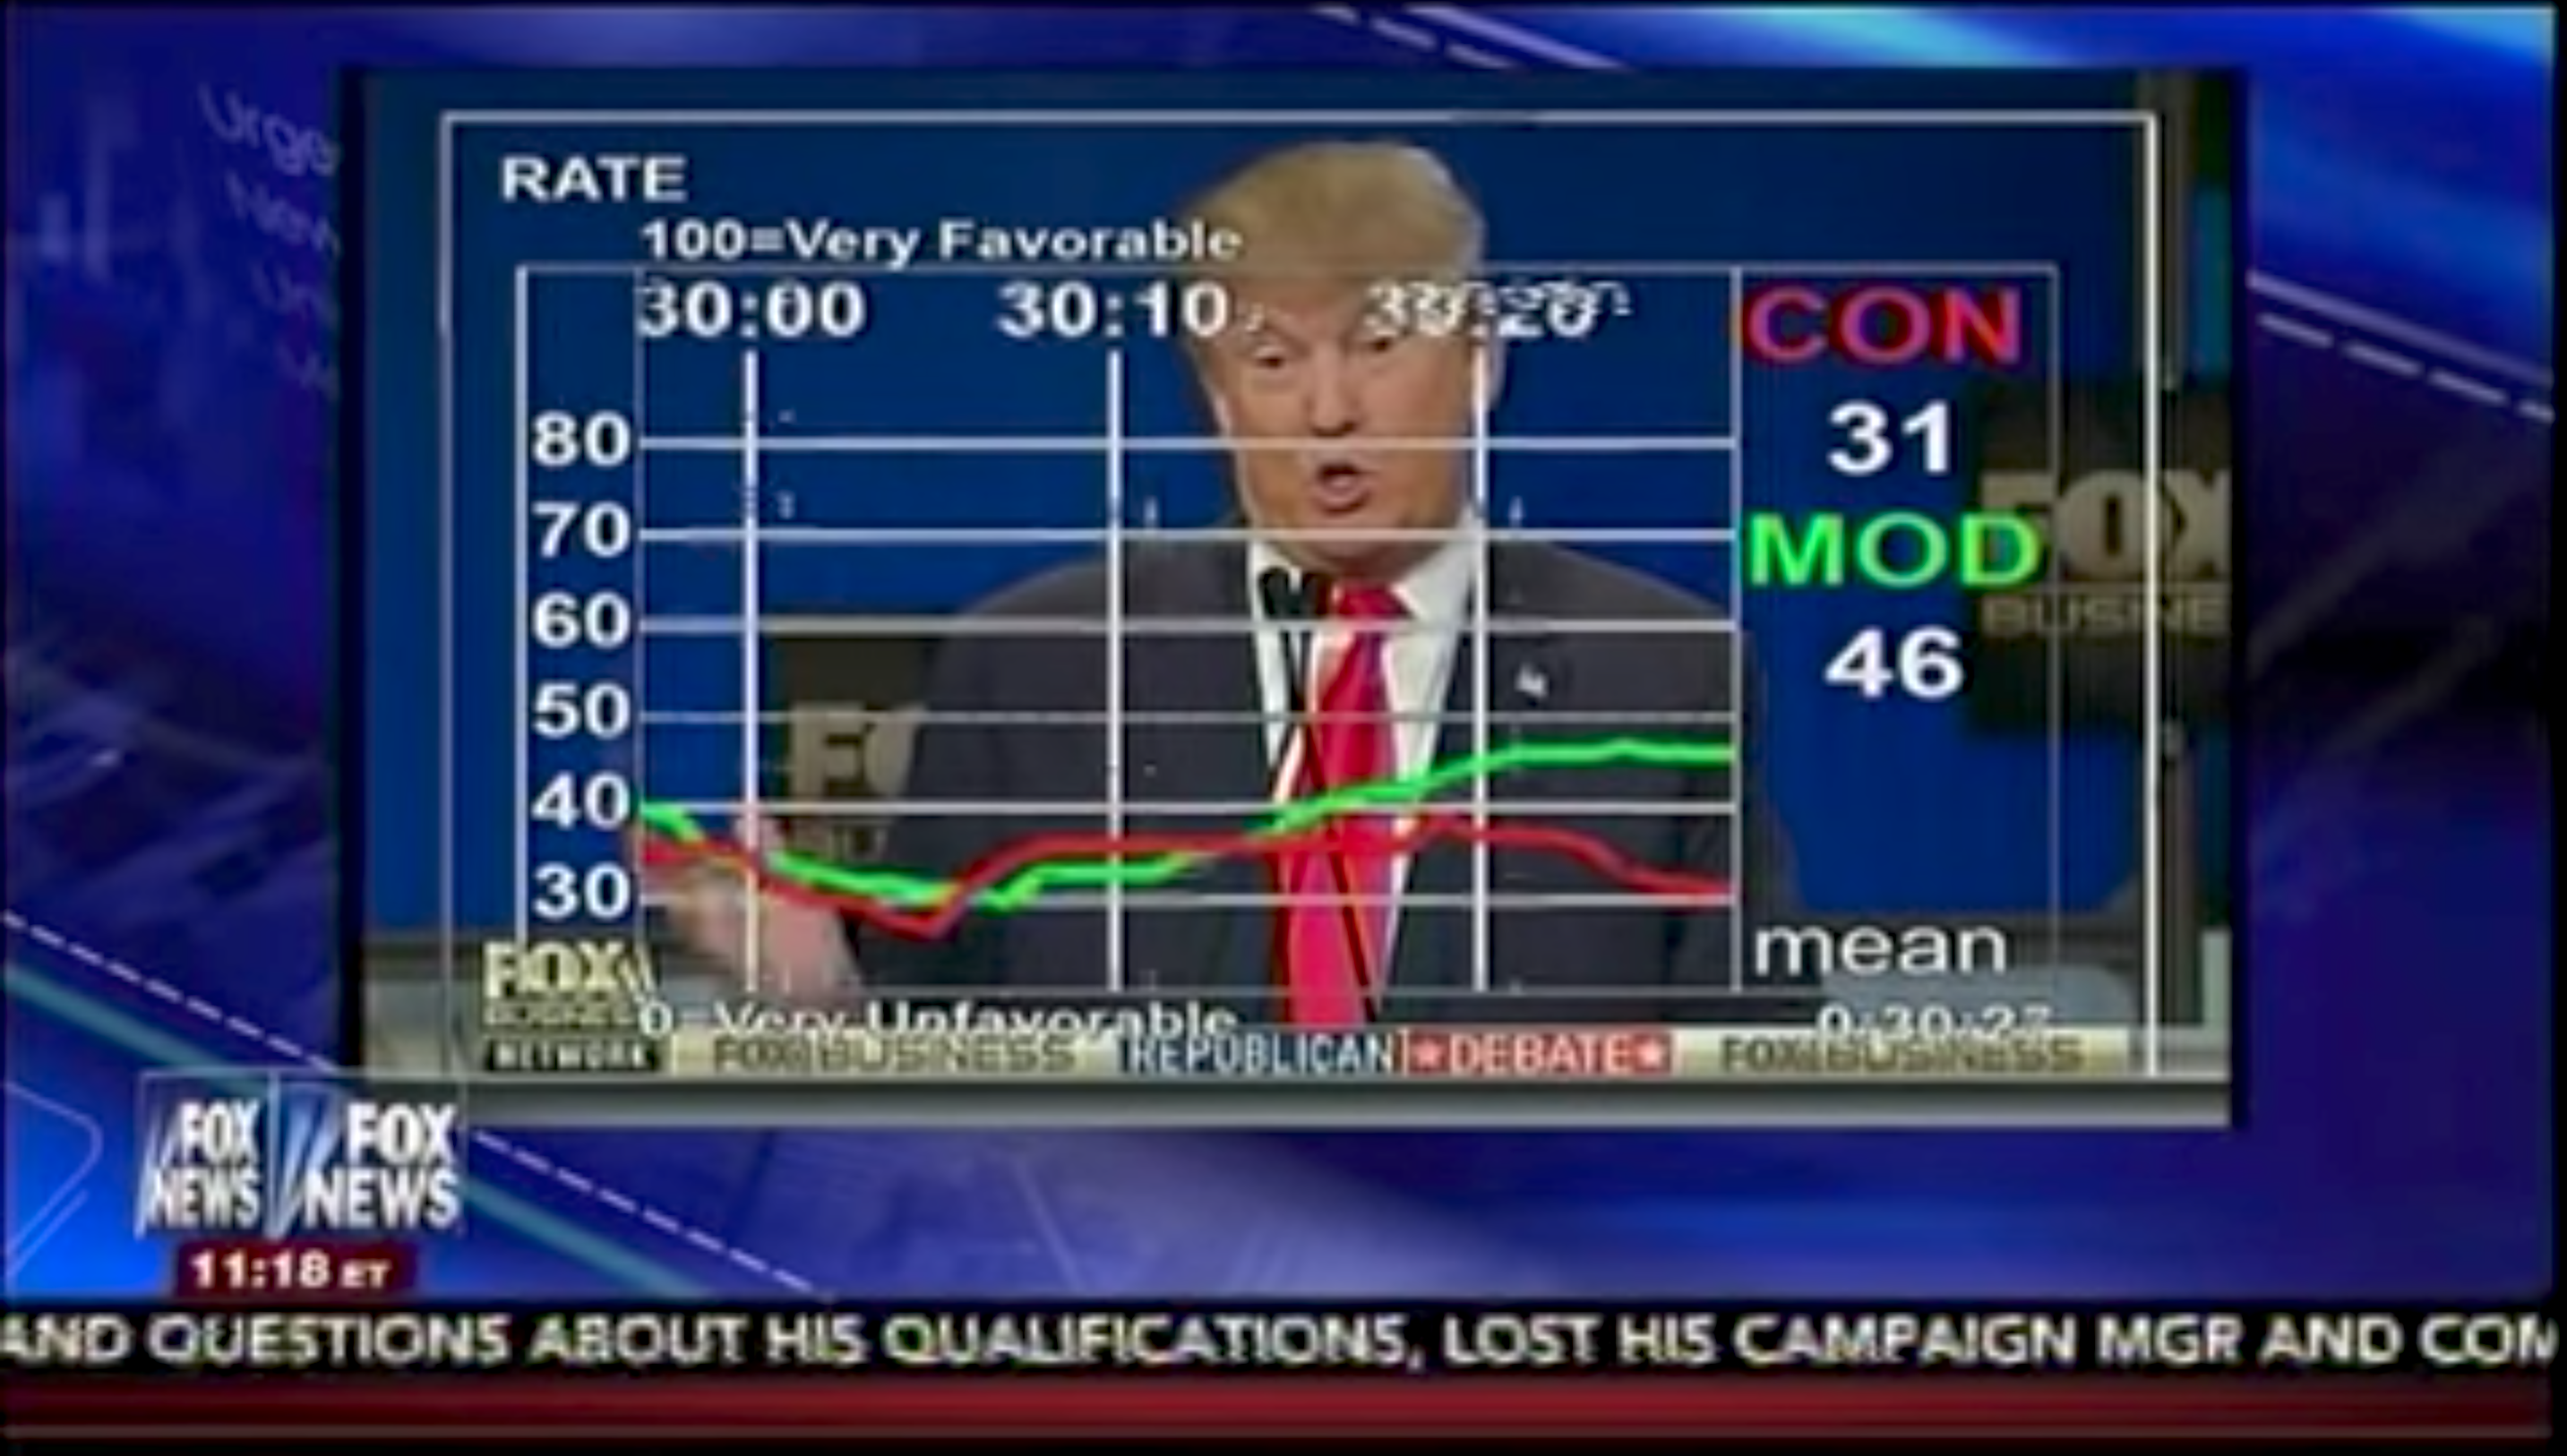
\includegraphics[width=\textwidth]{chapters/6/fig/pollester.png}               
 	 \caption{method for continuous input}
  	\label{fig:poll}
\end{marginfigure}
This app had focused on bikers, and did not take into account people who use other modes of transportation, such as pedestrians or car drivers. It is important to incorporate input from diverse people, and this both applies to the analytical and synthetic phase. It is easy to imagine to discuss the prioritization side, but the data on on-bike reports be should capture in a simulated environment.
Using a VR headset can simulate the bike ride and solicit data from people using a virtual environment projecting recorded material of one commute.




\subsection{How to tackle "relative" valuing}
Multiple people have commented the relativeness of their perception. Data shows that they feel insecure when bike lanes disappear. Using a gradational input like a volume knob will be suitable for getting a continuous input. The users feedback also cast new questions on how to annotate the city. Bikebump used a 15m radius geofence as a method, but users implied that 'good' situations are likely to be a continuous experience rather than a pulsive reaction. Looking at a constant input may also validate this perception.


\subsection{Incentivasation}
Shirkey has mentioned the internet have lowern There are two kinds of value mechanisms in a collective action. \cite{shirky2010cognitive}
distributed donation matching system \\
method for periodic participation - donation matching system \\
% combining for post / pre natural / artificial disasters
\subsection {update infrastructure for autonomous vehicles}
use this renovation opportunity for making cities compatible with autonomous vehicles (PEV)
\subsection{Headphones w/ noise cancellation for collecting sound from both
sides}
% TODO: incomplete
\subsection{Holacracy and liquid democracy}
% TODO: incomplete

\section{Concluding Remarks}
\cite{rudofsky1964architecture}


 

\appendix
% \chapter{Appendix A. (Un)structured method of traditional community engagement methods}
\label{app:traditional}

\begin{table*}
\centering
\begin{tabular}{|m{15em}|c|c|c|}
Method & Procedure & Output & Evaluation \\
\toprule
Planning for Real & yes & yes & yes \\
Citizens' Panels & yes & yes & yes \\ 
Community Surveys & yes & yes & yes \\
Community Mappings & no & yes & yes \\
Future Search & yes & yes & no \\
Open Space Technology & yes & no & no \\
Citizens' Juries & no & yes & no \\
Public Meetings & no & yes & no \\
Workshops and Focus Groups & no & no & no \\
Forums & no & no & no \\
Roundtable / Consensus Building & no & no & no \\
Street Stalls & no & no & no \\
\end{tabular}
\caption{structured method for community engagement}
\label{tab:traditional_method}
\end{table*}

\clearpage
\newpage

% \chapter{Appendix A}

\clearpage
\newpage

% \chapter{Appendix C. Questions asked after the fixed route trial and
proposal section}

\label{appc:afterquestions}

\section{After the bike ride}
\begin{enumerate}
\item Did everything work as expected?
\item Tell me the places that you felt danger.
\item For example, there two locations were the place it recently had accidents. 
\item Tell me the places that you felt safe.
\item Did the app make you more conscious about road safety? 
\section{Before showing the synthetic side}
\item Do you know the proper procedure to propose or send a petition if you want to change a portion of the city?
\section{After showing the synthetic side}
\item Did the app make you feel agency or your data represents what you want?
\item One thing we wanted to know about this experiment is about the procedure. It has two stages, the analytical and synthetic side. Did you feel your reporting and was it different when you were proposing. 
\item Do you see any advantages having the data collection visualization and proposals and voting in the same platform? What is different than having it separately?
\item Do you think the public will appreciate it and people will use this app in a real context?
\item I'm thinking there are two main ways to use this app. One situation
  is to have the city define a road to concentrate and have volunteers pass
  and put reports and improvement plans. The other is the unlimited, which
  citizen has full freedom to report and propose where ever they want.
\end{enumerate}
\clearpage
\newpage

% \chapter{Appendix D. Biking behavior and passive observation}

\begin{longtable}{|c|c|c|c|c|}
\hline
id & mount? & direction & wait & others \\
\toprule
1 & no & boston & 0 & \\ \hline 
2 & no & boston & 0 & \\ \hline
3 & no & cambridge & 0 & \\ \hline
4 & no & cambridge & 0 & \\ \hline
5 & no & cambridge & 0 & approach from wrong side \\ \hline
6 & no & cambridge & 0 & \\ \hline
7 & no & cambridge & 0 & \\ \hline
8 & no & cambridge & 0 & \\ \hline
9 & no & boston & 0 & \\ \hline
10 & no & boston & 60 & looked at phone from pocket \\ \hline
11 & yes & boston & 10 & passed near center line \\ \hline
12 & yes & boston & 0 & \\ \hline
13 & yes & boston & 20 & \\ \hline
14 & no & cambridge & 0 & \\ \hline
15 & yes & cambridge & 5 \\ \hline
16 & no & boston & 0 & \\ \hline
17 & no & boston & 0 & \\ \hline
18 & no & boston & 0 & hubway \\ \hline
19 & no & boston & 0 & hubway \\ \hline
20 & no & boston & 0 & \\ \hline
21 & no & boston & 0 & \\ \hline
22 & no & boston & 0 & with dog \\ \hline
23 & no & boston & 0 & \\ \hline
24 & no & boston & 0 & \\ \hline
25 & no & boston & 0 & passed near center line \\ \hline
26 & no & cambridge & 0 & \\ \hline
27 & no & cambridge & 0 & \\ \hline
28 & no & boston & 0 & \\ \hline
29 & no & boston & 0 & \\ \hline
30 & no & boston & 0 & \\ \hline
31 & yes & boston & 0 & \\ \hline
32 & yes & boston & 0 & \\ \hline
33 & no & boston & 5 & waited  \\ \hline
34 & yes & boston & 0 & one side walk operating smartphone \\ \hline
35 & no & boston & 0 & \\ \hline
36 & no & boston & 10 & \\ \hline
37 & no & boston & 0 & hubway, operating smartphone \\ \hline
38 & yes & cambridge & 0 & \\ \hline
39 & yes & cambridge & 0 & approach from wrong side \\ \hline
40 & no & boston & 0 & pushing bike in intersection \\ \hline
41 & no & cambridge & 0 & approach from wrong side \\ \hline
42 & no & cambridge & 0 & approach from wrong side \\ \hline
43 & no & boston & 0 & \\ \hline
44 & no & boston & 20 & hubway \\ \hline
45 & no & boston & 0 & \\ \hline
46 & no & boston & 0 & hubway \\ \hline
47 & no & boston & 0 & \\ \hline
48 & no & boston & 0 & \\ \hline
49 & no & boston & 0 & \\ \hline
50 & no & boston & 0 & \\ \hline
51 & no & cambridge & 0 & sidewalk \\ \hline
52 & no & boston & 0 & \\ \hline
53 & no & cambridge & 30 & u-turn \\ \hline
54 & no & cambridge & 20 & \\ \hline
55 & no & cambridge & 0 & \\ \hline
56 & no & cambridge & 0 & \\ \hline
57 & no & boston & 0 & \\ \hline
58 & no & boston & 0 & \\ \hline
59 & no & boston & 0 & \\ \hline
60 & no & boston & 0 & hubway \\ \hline
61 & no & boston & 0 & \\ \hline
62 & yes & cambridge & 0 & \\ \hline
63 & no & cambridge & 0 & \\ \hline
64 & no & boston & 5 \\ \hline
65 & no & boston & 0 & \\ \hline
66 & no & boston & 0 & hubway \\ \hline
67 & no & boston & 0 & \\ \hline
68 & no & boston & 0 & \\ \hline
69 & no & boston & 0 & \\ \hline
70 & no & boston & 5 & push bike to cross \\ \hline
71 & no & boston & 0 & hubway \\ \hline
72 & no & boston & 0 & wrongside \\ \hline
73 & no & boston & 0 & \\ \hline
74 & no & boston & 0 & \\ \hline
75 & no & boston & 0 & \\ \hline
76 & no & cambridge & 0 & \\ \hline
77 & no & cambridge & 0 & family \\ \hline
78 & no & cambridge & 0 & family \\ \hline
79 & no & cambridge & 0 & family \\ \hline
80 & no & boston & 0 & \\ \hline
81 & no & cambridge & 0 & \\ \hline
82 & no & cambridge & 0 & \\ \hline
83 & no & cambridge & 0 & \\ \hline
84 & no & boston & 0 & \\ \hline
85 & no & cambridge & 0 & \\ \hline
86 & no & boston & 0 & \\ \hline
87 & no & cambridge & 0 & \\ \hline
88 & no & boston & 0 & \\ \hline
89 & no & boston & 30 & \\ \hline
90 & no & boston & 0 & hubway \\ \hline
91 & no & boston & 0 & hubway \\ \hline
92 & no & boston & 0 & hubway \\ \hline

\caption{static observation}
\label{tab:static_observation}
\end{longtable}


\clearpage
\newpage

%% This defines the bibliography file (main.bib) and the bibliography style.
%% If you want to create a bibliography file by hand, change the contents of
%% this file to a `thebibliography' environment.  For more information 
%% see section 4.3 of the LaTeX manual.
\begin{singlespace}
\bibliography{main}
\bibliographystyle{apalike}
\end{singlespace}

\end{document}

